\documentclass{Quintorthesis} 

\usepackage[utf8]{inputenc}
\usepackage{colortbl}
\usepackage[export]{adjustbox}
\usepackage{booktabs}
\usepackage{graphicx, hyperref, parskip, subcaption, float, fancyhdr, amsmath, mathtools, wrapfig, color, titlesec }
\usepackage[dutch]{babel}
\usepackage{listings}
\usepackage{enumitem}
\usepackage[font={small, it}]{caption}
\usepackage[toc,page]{appendix}
\usepackage[natbibapa]{apacite}
\usepackage{pdfpages}
\usepackage[acronym]{glossaries}
\usepackage{glossary-mcols}
\usepackage{bookmark}

\newcommand{\source}[1]{\caption*{Source: {#1}} }
\newcommand{\R}{\mathbb{R}}
\newcommand*{\Scale}[2][4]{\scalebox{#1}{$#2$}}%

% Gherkin definition %

\lstdefinelanguage{Gherkin}{
  keywords={When, Then, Given, And},
  ndkeywords={Feature, Scenario},
  sensitive=false,
  comment=[l]{\#},
  morestring=[b]',
  morestring=[b]"
}

\setglossarystyle{mcolindexgroup}
\makenoidxglossaries
\loadglsentries{begrippen}

\begin{document}
  \baselineskip=15pt plus1pt
  \parskip=15pt
  \setcounter{secnumdepth}{2}
  \setcounter{tocdepth}{2}

  \renewcommand\appendixpagename{Bijlages}
  \renewcommand\appendixtocname{Bijlages}
  \newcommand{\hsp}{\hspace{10pt}}

  % Custom spacings for chapter, paragraph and textcolors
  \titleformat{\chapter}[hang]{\Huge\bfseries}{\thechapter\hsp\textcolor{quintorred}{|}\hsp}{0pt}{\LARGE\bfseries}
  \titlespacing*{\chapter}{0pt}{0pt}{20pt}
  \titlespacing*{\paragraph}{0pt}{0pt}{10pt}

  \begin{titlepage}
    \documenttype{Onderzoek naar} 
    \title{Gedistribueerde netwerken en identiteit binnen Blockchain technologie}
    \author{Jeffrey van Hoven}
    \date{\today}
    \maketitle
  \end{titlepage}

  % Start of Roman Pages. Here goes the preface, definitions 
  % and abstract
  \begin{romanpages}
    \chapter*{Voorwoord}

Voor u ligt mijn afstudeerverslag; ``\textit{Het realiseren van een gedistribueerd netwerk met mogelijkheid tot identiteit management ter behoeve van Blockchain technologie}'' waarin ik schrijf over de uitvoering van het onderzoek dat gedaan is ten behoeve van mijn afstuderen voor de opleiding Informatica aan de Haagse Hogeschool. Het betreft verslaglegging van het proces dat doorlopen is om de uitdagende opdracht zoals voorgesteld door Quintor uit te voeren.

In de opdracht is er na uitvoerig onderzoek tot de conclusie gekomen welke technieken geschikt zijn om toegepast te kunnen worden om de Blockchain onderdelen Distributed Network en Identity Management te realiseren. Gedurende het afstudeertraject kon ik altijd met vragen terecht bij zowel mijn bedrijfsbegeleider, Ben Ooms, als de Blockchain expert, Pim Otte.

Hierbij bedank ik mijn begeleiders, vanuit Quintor en vanuit de opleiding, voor hun begeleiding, inzichten en ondersteuning tijdens het afstudeertraject. Daarnaast wil ik graag mijn mede afstudeerders bedanken voor hun meedenken en inzichten in het vinden van oplossingen. In het bijzonder bedank ik mede afstudeerder Kevin Bos, waarmee de samenwerking gedurende de opdracht aangenaam en productief is geweest. 

Als laatste bedank ik mijn familie en vrienden voor hun ondersteuning, indirect of direct, niet alleen tijdens het afstuderen, maar ook tijdens mijn studieloopbaan. Zonder hun ondersteuning zou dit mogelijk geweest zijn.

Ik wens u veel leesplezier toe.

\bigskip
\bigskip

Jeffrey van Hoven \\
Den Haag, 1 juni 2018

    \tableofcontents     
    \listoffigures              
    \listoftables
    \printnoidxglossary[title=Woordenlijst]
    \printnoidxglossary[title=Afkortingen, type=\acronymtype]
  \end{romanpages}

  \chapter{Inleiding}

Dit verslag is geschreven in het kader van mijn afstudeeropdracht bij Quintor en dient ter beoordeling van de werkzaamheden die uitgevoerd zijn voor de bachelorstudie Informatica aan de Haagse Hogeschool. 

Door de snelle groei van het Blockchain domein heeft Quintor in 2017 in samenwerking met DUO/MinOCW, Groningen Declaration Network, Stichting ePortfolio Support, TNO en Rabobank, het Blockchain Field-lab Education gestart in Groningen. Het Blockchain-lab is opgezet om expertise en kennis uit te wisselen op regionaal, nationaal en internationaal gebied. De oprichting van het Blockchain Field-lab Education heeft er mede voor gezorgd dat Quintor meer kennis wilt opdoen over het Blockchain domein om zo inzicht te krijgen in hoe Blockchain technologie ingezet kan worden binnen vraagstukken vanuit klanten. 

In hoofdstuk 2 is de organisatie beschreven waar het afstudeertraject heeft plaatsgevonden. Vervolgens wordt in hoofdstuk 3 de opdracht gepresenteerd. In hoofdstuk 4 wordt de aanpak van de opdracht onderbouwd en in hoofdstuk 5 wordt de orientatie van de opdracht besproken. In hoofdstuk 6 worden de werkzaamheden van het vooronderzoek besproken waarin de basis van Blockchain technologie ter sprake komt. In hoofdstuk 7 wordt het hoofdonderzoek naar de segmenten Identity Management en Distributed Network in bestaande Blockchain implementaties beschreven. Hoofdstuk 8 presenteert het advies dat gegeven wordt naar aanleiding van het gedane onderzoek. Hoofdstuk 9 beschrijft de totstandkoming van het ontwerp voor de architectuur. In hoofdstuk 10 worden de keuzes die gemaakt zijn voor de indeling van het Proof of Concept beschreven en wordt er kort uitgelicht hoe de realisatie van het Peer-to-Peer netwerk is verlopen. In hoofdstuk 11 wordt er geëvalueerd over de producten, de aanpak, de geselecteerde beroepstaken, het functioneren in het bedrijf en de leerpunten die getrokken zijn uit het project. Tot slot worden er in hoofdstuk 11 aanbevelingen gegeven voor vervolgonderzoek.

  \chapter{Quintor}
\textit{In dit hoofdstuk zal er inzicht gegeven worden over het bedrijf Quintor waar het afstudeerproject heeft plaatsgevonden. Er wordt verteld over de diensten die Quintor levert en wat de doelen zijn van de organisatie. Er zal ook kort toegelicht worden waar de afstudeerder binnen het bedrijf opereert en welke werknemers vanuit Quintor betrokken zijn bij de afstudeeropdracht.
}

Quintor is een toonaangevend bedrijf op het gebied van Agile software development, Enterprise Java / .NET technologie en mobile development. Het bedrijf is begonnen in 2005 in Groningen en is opgericht door Johan Tillema, de huidige CEO van het bedrijf. Sinds 2005 heeft het bedrijf een gezonde groei doorgemaakt en heeft inmiddels 150 medewerkers, verspreid over vestigingen in Groningen, Amersfoort en Den Haag. Vanuit deze vestigingen ondersteunt het bedrijf klanten bij de uitdagingen die grootschalige Enterprise projecten met zich meebrengen. Het succes van Quintor is te danken aan drie pijlers: techniek en architectuur, een hoogwaardige ontwikkelstraat en het Agile/Scrum proces. Tevens beschikt Quintor over een Software Factory waarin in-house projecten voor klanten worden uitgevoerd.

\section{Software Factory}

In de Software Factory staat alle kennis en expertise die Quintor heeft verzameld over de jaren heen. Het is een hoogwaardig platform waarin de tooling, standaarden en best practices en tevens een complete oplossing is voor het managen en hosten van Scrum projecten. Dit wordt onder andere gebruikt om klanten te helpen bij het professionaliseren en efficiënter inrichten van softwareontwikkeling. Een groot deel van de werkzaamheden die Quintor dan ook uitvoert voor klanten is consultatie bij o.a. het implementeren van Agile/Scrum werk- en denkwijze. Naast Java en .NET development behoort ook mobile development tot de kerncompetenties van Quintor, en is dan ook opgenomen in de Software Factory. Hieronder zijn een aantal onderdelen uitgelicht die voorkomen in de Software Factory.

\paragraph{Enterprise architectuur}

Vanuit een pragmatische insteek en op basis van jarenlange ervaring helpen de software architecten van Quintor organisaties bij het maken van de juiste keuzes op het gebied van architectuur. Hierbij gaat het om het zowel opstellen als implementeren van een architectuur.

\paragraph{Informatie analyse}

Het in kaart brengen van informatie door het gebruik van diverse analyse- en ontwerptechnieken zoals UML, user-stories en use-cases in een Agile omgeving.

\paragraph{Java en .NET development}

Het realiseren van duurzame IT-systemen, in-house of bij klanten, die naadloos aansluiten bij de wensen van de business. Hierbij zijn er een groot aantal van omvangrijke systemen ontwikkelt.

\paragraph{Agile/Scrum}

Agile/Scrum is een effectieve en flexibele methode die uitgaat van een iteratiefontwikkelproces. Het trainen van complete projectteams met een op maat gemaakte training, waarbij aansluitend support en coaching gegeven wordt.

\paragraph{Mobile development}

Mobiele applicaties voor iPhone, iPad en Android. Specifiek hiervoor is het 'Mobile development center' opgezet, waarin er apps ontworpen, ontwikkelt en beheert worden. Dit betreft de realisatie van stand-alone tot volledige geïntegreerde Enterprise apps.

\section{Visie}

Een van de doelstellingen die Quintor heeft is het professionaliseren van software development. Aansluitend daarop probeert het bedrijf continu voor te lopen op de concurrentie door het opdoen van kennis op het gebied van nieuwe technologieën, waarbij professionalisering van de werkwijze voorop staat.

\begin{formal}
  \label{visie}
  ``Onze ambitie: professionaliseren van software development."
  \\ Johan Tillema, Chief Executive Officer
\end{formal}

Door het aanbieden van uitdagende afstudeeropdrachten wordt er kennis opgebouwd die benodigd is om nieuwe technologieën, zoals bijvoorbeeld Machine Learning of Blockchain, in te zetten om klanten te adviseren bij de uitdagingen die grootschalige Enterprise projecten met zich meebrengen en zal, middels het volwassen genoeg is, opgenomen worden in de Software Factory.

\section{Organisatie}
In fig. \ref{organogram} wordt de organisatie van Quintor weergegeven. Bovenaan staat Johan Tillema, de oprichter en CEO. Direct eronder staat het Secretariaat en het Recruitment Office. Hierin is te zien dat er vier segmenten zijn waarop er consultatie aangeboden wordt: development, analysis en design en front-end.

\begin{figure}[h]
  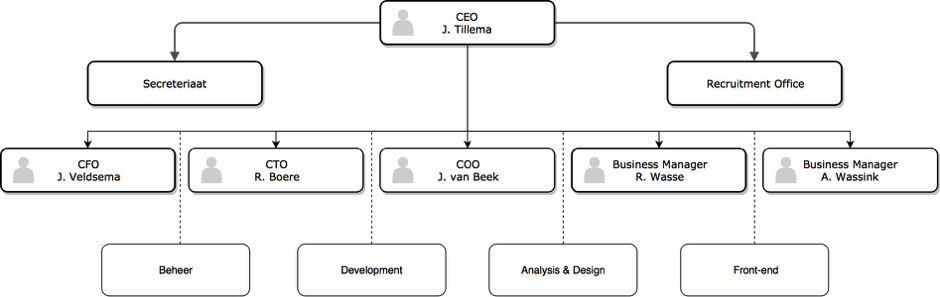
\includegraphics[width=1\textwidth]{figures/organogram}
  \caption{Organogram van Quintor.}
  \label{organogram}
\end{figure}

\newpage
Zelf val ik onder het development segment, waarbij er aangestuurd wordt door Ben Ooms, (beschreven in \ref{begeleider}). Er wordt zelfstandig gewerkt aan de opdracht waarbij er een aantal praktijken van Scrum toegepast zijn tijdens het afstudeertraject. Zo is er elke twee weken een zogenaamde demo dag waarbij iedere afstudeerder een demonstratie over waar hij of zij de afgelopen tijd mee bezig is geweest, en of er ergens tegenaan gelopen wordt zodat er samen nagedacht kan worden over mogelijke oplossingen.

\section{Infrastructuur}

Quintor maakt intensief gebruik van het Agile principe en dit is dan ook terug te vinden in de infrastructuur die ingericht is voor de consultanten binnen Quintor. Voor het uitvoeren van projecten wordt Atlassian JIRA gebruikt om het Agile proces te ondesteunen. Hierin is het mogelijk om taken te creëren en toe te wijzen aan projecten. Elke taak is dan individueel op te pakken door een team die op een bepaald project gezet is. 

Voor het waarborgen van de kwaliteit van de software wordt er gebruik gemaakt van Atlassian BitBucket. BitBucket is een web-based versiebeheer systeem dat het Mercurial of Git revisiesystemen ondersteund. Daarnaast werkt het uitstekend samen met JIRA, waarbij het mogelijk is om naar taken die opgepakt zijn binnen JIRA te refereren binnen BitBucket.

Communicatie binnen de organisatie gaat via het interne mail-systeem die functionaliteiten ondersteund zoals bijvoorbeeld het interne chat-systeem waarbij het mogelijk is om elke medewerker te benaderen en een kalender die het mogelijk maakt om afspraken te koppelen aan medewerkers en locaties.

\section{Betrokkenen}

Binnen Quintor zijn er een aantal medewerkers die nodig zijn om het project tot een geslaagd einde te brengen. Hieronder zijn deze medewerkers kort benoemd en wat hun rol is binnen het afstudeertraject.

\paragraph{Ben Ooms} \label{begeleider} is de teamleider van Quintor Den Haag en is tevens de begeleider tijdens het afstudeertraject. Zijn uitvoerende taken hierbij zijn dan ook onder andere advies geven over de aanpak van de opdracht en waarbij mogelijk de voortgang van de opdracht te waarborgen.

\paragraph{Pim Otte} \label{expert} is de Blockchain expert binnen Quintor en heeft veelal ervaring met de toepassing en realisatie van applicaties die gebruik maken van Blockchain technologie. Hij is beschikbaar gedurende de afstudeeropdracht om inzichten en feedback te geven op de uitgevoerde werkzaamheden.

\paragraph{Kevin Bos} is afstudeerder afkomstig van Avans Hogeschool. Hij is verantwoordelijk voor het lokale gedeelte van de Blockchain opdracht. Tijdens de afstudeeropdracht is hij een stakeholder van het project en zal er een zekere mate van samenwerking aanwezig zijn.
  \chapter{Opdracht}

In 2017 heeft Quintor in samenwerking met DUO/MinOCW, Groningen Declaration Network, Stichting ePortfolio Support, TNO en Rabobank, het Blockchain Field-lab Education gestart in Groningen. Het Blockchain-lab is opgezet om expertise en kennis uit te wisselen op regionaal, nationaal en internationaal gebied. De oprichting van het Blockchain Field-lab Education heeft er mede voor gezorgd dat Quintor meer kennis wilt opdoen op het gebied van Blockchain. Daarnaast bestaat er de mogelijkheid dat het bedrijf in de toekomst Blockchain technologie wilt inzetten om vraagstukken vanuit klanten op te lossen.

\begin{figure}[h]
  \centering
  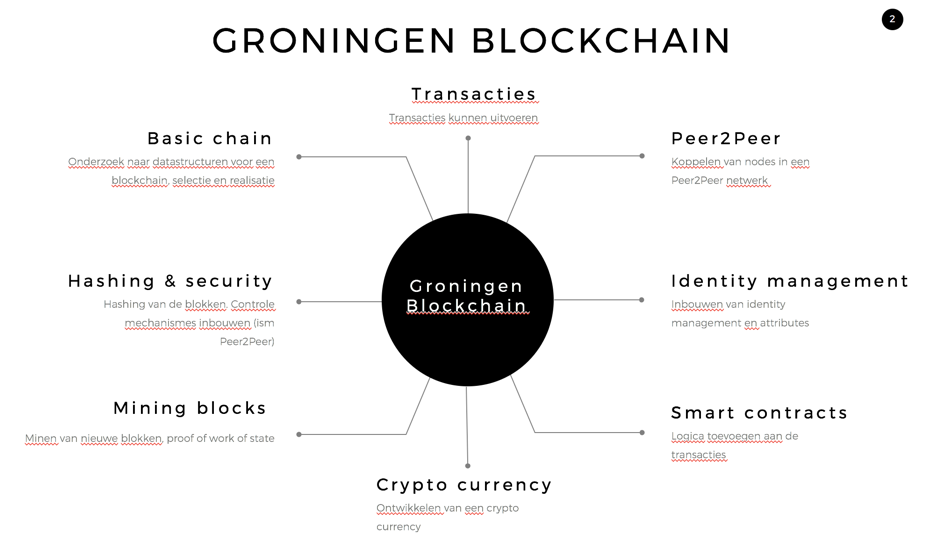
\includegraphics{figures/indeling_blockchain_opdracht}
  \caption{Indeling opdracht Blockchain ontwikkeling zoals gegeven door Quintor afkomstig uit.}
  \label{indeling_blockchain_opdracht} 
\end{figure}

De focus in de afstudeeropdracht ligt op de Blockchain onderdelen Identity Management en Peer2Peer (Distributed Network). Dit zal in samenwerking gaan met een andere afstudeerder, Kevin Bos, die verantwoordelijk is voor de onderdelen Basic chain, Hashing \& security en Mining blocks. 

\newpage
\section{Probleemstelling}

Sinds de opkomst van Bitcoin is de Blockchain technologie, de techniek die het mogelijk maakt om het op een gedecentraliseerde manier te laten werken, steeds populairder geworden. Alhoewel de Blockchain-technologie nog in de kinderschoenen staat, gaan de ontwikkelingen in het domein zeer snel. Zo worden er toepassingen bedacht die niet alleen voor de financiële markten interessant zijn, maar ook voor bijvoorbeeld het digitaliseren van contracten en contractbeheer.

Aangezien de toepassing en adoptie van Blockchain technologie steeds groter wordt wil Quintor de toepassingsmogelijkheden en technieken onderzoeken om zo inzicht te kunnen krijgen in hoe het gebruikt kan worden in de aangeboden vraagstukken vanuit klanten.

\section{Doelstelling}

De doelstelling van de opdracht is verspreid over onderdelen van Blockchain technologie, zoals te zien in fig. \ref{indeling_blockchain_opdracht}. Hierdoor is er een globaal doel en een doel die specifiek voor deze opdracht geldt. Het streven naar het globale doel is het opdoen van kennis omtrent het realiseren van een Blockchain implementatie. Het doel van deze specifieke opdracht is middels het opstellen van een proof-of-concept van de Blockchain onderdelen Identity Management en Distributed Network, zonder gebruik te maken van bestaande Blockchain protocollen, kennis te ontwikkelen voor Quintor op het gebied van Blockchain technologie.

\section{Resultaat}

Indien de opdracht succesvol afgerond is, zijn de onderdelen Identity Management en het Peer2Peer netwerk gerealiseerd aan de hand van voorgestelde technieken die voortgekomen zijn uit het gedane onderzoek. In samenwerking met de onderdelen die gerealiseerd zijn door Kevin Bos zal er een werkend Proof of Concept van een Blockchain gerealiseerd zijn. Zowel het Proof of Concept als het onderzoek zal voor Quintor inzicht bieden in het Blockchain domein en de ontwikkelingen daarin.

\subsection{Producten}

Als onderdeel van de afstudeeropdracht zullen er verschillende producten worden opgeleverd aan Quintor en aan de Haagse Hogeschool. Deze staan hieronder gespecificeerd.

De op te leveren producten aan Quintor zijn:
\begin{itemize}
  \item{Adviesrapport}
  \item{Sprint demo presentaties}
  \item{Broncode van de ontwikkelde applicatie}
  \item{Opgestelde documentatie}
\end{itemize}

De op te leveren producten aan de Haagse Hogeschool zijn:
\begin{itemize}
  \item{Afstudeerscriptie}
  \item{Plan van Aanpak}
  \item{Adviesrapport}
  \item{Testrapport}
  \item{Technisch ontwerp}
\end{itemize}



  \chapter{Oriëntatie}

\textit{Dit hoofdstuk beschrijft het proces van de benodigde inventarisatie om duidelijkheid te krijgen over de criteria die gesteld zijn in de originele opdracht. Het doel van het uitvoeren van de inventarisatie is het opstellen van requirements en/of criteria die gesteld zijn aan het onderzoek en het uiteindelijke Proof of Concept.}

Zoals eerder besproken bevat de opdrachtomschrijving criteria die nader gespecificeerd dienen te worden. Deze criteria gaan over snelheid, beveiliging en toepassingsmogelijkheden waarbij elke invulling van deze criteria mogelijk invloed heeft op de planning en/of de aanpak van het project. Een van de belangrijkste criteria hierbij is de toepassingsmogelijkheid voor het Proof of Concept, waarbij er rekening gehouden moet worden met benodigde domeinkennis die het vooronderzoek en/of onderzoek kunnen uitbreiden.

Deze mogelijke implicaties zijn dan ook de aanleiding geweest tot een serie van gesprekken met de Blockchain expert en de bedrijfsbegeleider binnen Quintor, waarin er geprobeerd is een juiste toepassing te vinden die gerealiseerd kon worden binnen de beperkte tijd.

\section{Omwenteling en implicaties}

Uit deze gesprekken is voortgekomen dat de toepassing van het Proof of Concept los staat van de uitvoering van het onderzoek, aangezien de toepassing alleen maar dient als bewijs dat de gerealiseerde Blockchain kern functioneert. Dit heeft ertoe geleid dat er beslist is over veranderingen die impact hebben op de insteek van de opdracht zoals het origineel opgesteld was. Hieronder zijn kort de veranderingen weergegeven.

%TODO: Omwenteling opdracht

\subsubsection{Generieke Blockchain} 
Er is besloten dat voor het Proof of Concept en het onderzoek de focus zal liggen op het creeren van een generieke Blockchain. Daarbij is ook het besluit genomen om de toepassing van het Proof of Concept bij het adviesrapport te betrekken. Zelf had ik hierbij mijn twijfels aangezien `generiek' ook gezien kan worden als een eis aan de implementatie, niet als een eis op de vorm en uitvoering van het onderzoek. 

Deze twijfel is dan ook aangekaart in de sprintreview, waarbij er besloten is dat dit deze eis inderdaad aan de implementatie gesteld is en niet aan het onderzoek. Dit heeft als gevolg dat de term `generiek' niet voorkomt in het onderzoek en het niet wenselijk om een dergelijk aspect als criteria voor de selectie van de implementaties te gebruiken.

\subsubsection{Criteria}

Er is besloten dat de criteria behandeld zal worden in het onderzoek, waardoor de grootte van het onderzoek zal toenemen. De toepassingsmogelijkheid zal hierbij geadviseerd worden in het adviesrapport. Hieruit zal beslist worden welke toepassing gerealiseerd kan worden binnen de beperkte tijd.
  \chapter{Aanpak}
\label{Aanpak}

\textit{In dit hoofdstuk wordt de totstandkoming van de aanpak voor de opdracht besproken. Het gaat uit van de beginsituatie zoals beschreven in het afstudeerplan, in te zien in bijlage \ref{appendix:afstudeerplan}. Daarnaast worden de afwijkingen besproken tegenover de originele opdracht, zoals geformuleerd in hoofstuk 3.}

\section{Inrichting}

Aangezien Quintor een groot voorstander is van het Agile werken zien zij ook graag het afstudeertraject in die vorm uitgevoerd worden. Tijdens de studie is er veel ervaring opgedaan met het Scrum framework dat het Agile principe ondersteund waardoor het een logische keuze is om de structuur van het project te bepalen. Omdat een groot gedeelte van het project bestaat uit het individueel uitvoeren van onderzoek zijn niet alle best practices overgenomen. 

De rollen binnen het scrum proces \citep{schwaber2011scrum} zijn als volgt gedefinieerd:
\begin{itemize}[noitemsep]
  \item \textbf{Scrum Master} - Ben Ooms
  \item \textbf{Product Owner} - Johan Tillema / Ben Ooms
  \item \textbf{Development Team} - Jeffrey van Hoven
\end{itemize}

Een sprint zal bestaan uit twee weken waarbij aan het eind van de sprint een demo van de huidige status van het project wordt gegeven aan de afstudeerbegeleider vanuit Quintor. Tijdens dit moment is het mogelijk om advies te krijgen over de uitvoering van de werkzaamheden of blokkades waar tegenaan gelopen wordt. Daarnaast wordt er onder de afstudeerders dagelijks een stand-up gehouden waarin zaken zoals de status van het project, welke werkzaamheden gepland staan voor de dag en of er obstakels zijn besproken worden.
\subsection{Fases}

Er wordt uitgegaan van drie fases binnen het project: \textbf{onderzoek}, \textbf{ontwerp} en \textbf{realisatie}, waarbij de fases ontwerp en realisatie Agile uitgevoerd worden volgens de Scrum richtlijnen.

\newpage
\section{Fase 1: Onderzoek}
\subsection{Vooronderzoek}

In het afstudeertraject wordt er met technologieën gewerkt welke onbekend zijn. Er is er dan ook voor gekozen om aan de hand van vooronderzoek kennis op te doen over het Blockchain domein. Er zal eerst onderzocht worden wat een Blockchain is waarna er ingegaan wordt op de toepassing van de techniek. Vervolgens zal er worden gekeken naar de architectuur van de Blockchain en uit welke componenten het bestaat. Uiteindelijk zal er kennis opgedaan worden voor de onderdelen Identity Management en Distributed Network om zo een afbakening te creëren van de onderdelen. Deze kennis zal gebruikt worden, in overleg met Quintor, om de opdracht vorm te geven en inzichten op te doen over de mogelijkheden met de opdracht.

\subsubsection{Dataverzameling}
Voor het opdoen van voorkennis zullen er gepubliceerde research papers, wiki’s en blogs gebruikt worden. Hierna zal er een selectie van Blockchain implementaties gemaakt worden die bestudeerd zullen worden in het onderzoek.
\subsection{Hoofdonderzoek}

Voor het uitvoeren van het onderzoek zal ik gebruik maken van deskresearch. Voor mijn deskresearch zullen er specifieke cases van Blockchain implementaties geanalyseerd worden op de segmenten Distributed Network en Identity Management. Hiervoor zal ik proberen een zo compleet mogelijk technische beschrijving van de werking van deze segmenten op te stellen.

In de opdrachtomschrijving die aangeleverd is door Quintor zijn er geen duidelijke eisen en specificaties gesteld aan zowel de uitvoering als realisatie van de afstudeeropdracht. Dit heeft ertoe geleid dat er een gesprek gehouden is met de Blockchain expert en de bedrijfsbegeleider over de eisen, afbakening en in welke mate de samenwerking met de andere afstudeerder benodigd zal zijn. Hieruit is naar voren gekomen dat er wederom geen specifieke eisen zijn en dat de afstudeerder onderzoek dient te doen naar implementaties om een zo goed mogelijk functioneel overzicht te creëren van de onderdelen die toegekend zijn. Omdat de missie van Quintor het vooroplopen op het gebied van IT ontwikkelingen is, is ervoor gekozen om exploratief onderzoek uit te voeren.

\section{Fase 2: Ontwerpen}
Uit het hoofdonderzoek zullen methoden en technieken geselecteerd worden die gerealiseerd zullen worden in een Proof of Concept. Alvorens deze gerealiseerd zal worden moet er nagedacht worden over hoe dit eruit zal komen te zien op technisch gebied. Het modelleren, implementeren en documenteren van een systeem vereist dat het systeem vanuit verschillende aspecten wordt bekeken. Er zal een keuze gemaakt worden betreft een methode voor het faciliteren van deze filosofie.


\section{Fase 3: Realisatie}
\subsection{Ontwikkeling}

De uitgekozen technieken zullen gerealiseerd worden in een Proof of Concept. Dit zal in samenwerking zijn met de andere afstudeerder, die het lokale gedeelte van de Blockchain ontwikkeld. De onderdelen dienen samen te werken tot een functionele Blockchain implementatie, waarbij er overlap zal zijn in de keuzes binnen de pakketselectie en realisatie.

\paragraph{Requirements} Er dienen criteria opgesteld te worden aan de hand van het resultaat van het onderzoek die van toepassing zijn op de realisatie van het Proof of Concept. Om te achterhalen wat de eisen en de toepassing waaraan het Proof of Concept moet voldoen zullen er informele interviews gehouden worden waarin requirements achterhaald worden.

\paragraph{Selecteren methoden} Voor het opzetten van een development workflow en de technieken die daarbij te pas komen in overeenstemming met Quintor zullen er beslissingen gemaakt worden op de manier waarop het Proof of Concept gerealiseerd gaat worden. Tevens zal hierbij gekeken worden naar de uitvoering van realisatie op bestaande implementaties.


% \subsection{Adviesrapport}
% TODO: Wat moet hiermee gebeuren?
% Om in overeenstemming met de opdrachtgever een toepassing te kiezen voor de functionaliteiten en/of technieken die onderzocht zijn in de geselecteerde protocollen, zal er een adviesrapport opgesteld worden waarin deze technieken en/of technologieën aangeraden worden. 

\clearpage
\section{Planning}
Er is een globale planning gemaakt die uitgaat van de drie gestelde fases: \textbf{onderzoek}, \textbf{ontwerp} en \textbf{realisatie}. Er wordt ervan uitgegaan dat elk van deze fases ongeveer \( \frac{1}{3} \)de van de tijd in beslag zal nemen. Aangezien de fases ontwerp en realisatie Agile uitgevoerd worden wordt er vanuit gegaan dat er niet veel tijd besteed zal worden aan het ontwerpen alvorens begonnen wordt aan de realisatie. Binnen deze drie fases zal er tijd gealloceerd worden voor het inventariseren, opzetten en opdoen van benodigde kennis en documentatie. In onderstaand tabel is een globale planning opgezet voor de drie fases.

\begin{table}[ht]
  \begin{tabular}{|p{6cm}|p{4cm}|p{4cm}|}
    \hline
    \textbf{Fase} & \textbf{Van} & \textbf{Tot en met} \\
    \hline
    Onderzoek & Week 3 & Week 9 \\
    \hline
    Ontwerp & Week 10 & Week 17 \\
    \hline
    Realisatie & Week 11 & Week 17 \\
    \hline
    Afronding & Week 18 & - \\
    \hline
  \end{tabular}
  \caption{Globale planning}
  \label{planning}
\end{table}

Waarbij de werkzaamheden die uitgevoerd zullen worden binnen een fase er ongeveer als volgt uitzien:

\begin{multicols}{2}
  \begin{itemize}[noitemsep]
    \item \textbf{Onderzoek}
    \begin{itemize}[noitemsep]
      \item Vooronderzoek
      \item Selectie implementaties
      \item Onderzoeksopzet
      \item Onderzoek
      \item Advies
    \end{itemize}
    \item \textbf{Ontwerp}
    \begin{itemize}[noitemsep]
      \item Selecteren methode
      \item Ontwerp individuele views
    \end{itemize}
    \item \textbf{Realisatie}
    \begin{itemize}[noitemsep]
      \item Informatieplan
      \item Realisatie in vorm van sprints
      \item Testen
    \end{itemize}
    \item \textbf{Afronding}
    \begin{itemize}
      \item Overdracht
      \item Afronding afstudeerverslag
    \end{itemize}
  \end{itemize}
\end{multicols}
  \chapter{Vooronderzoek en resultaten}

\textit{In dit hoofdstuk wordt er een introductie gegeven in het Blockchain domein. Deze kennis is benodigd om het onderzoek uit te voeren en om het Proof of Concept te realiseren. Daarnaast zal deze kennis helpen om de uitvoering van de opdracht te begrijpen. Het vooronderzoek dient tevens om overeenstemming te krijgen met de opdrachtgever over de richting van het onderzoek. Zoals verteld in de aanpak zijn er weinig eisen gesteld aan de uitvoering en toepassing van de afstudeeropdracht, waardoor het wenselijk is om een gezamenlijke overeenstemming te krijgen van wat mogelijk is met het onderzoek.}

Het vooronderzoek betreft kwalitatief-, exploratief onderzoek dat uitgevoerd wordt door middel van deskresearch. De reden dat ik hiervoor heb gekozen is omdat het Blockchain domein nieuw voor mij is en ik dus ook niet welke specifieke kennis ik nodig heb om de vragen te beantwoorden. De bronnen die ik gebruikt heb zijn zowel informeel als formeel waarbij er veel informatie afkomstig is uit het Bitcoin protocol, zoals beschreven door \cite{nakamoto2008bitcoin}. Dit is een van de meest gedocumenteerde Blockchain implementaties die publiekelijk in te zien is. Om de technische kennis te versterken voor de realisatie van het Proof of Concept is er een Coursera course gevolgd, Bitcoin and Cryptocurrency Technologies, waarin het Bitcoin protocol uitgelegd wordt. Dit is gevolgd omdat de beschrijving van het Bitcoin protocol niet meer toereikend is naar de huidige staat van de implementatie.

Er wordt ingegaan op de basis van Blockchain technologie waarna er gekeken wordt naar de mogelijke toepassingen. Vervolgens komt de architectuur van een Blockchain aan bod, waarbij de vraag ``Uit welke componenten bestaat een Blockchain implementatie?" wordt behandeld. Om een afbakening te maken voor het onderzoek wordt er gekeken naar wat de onderdelen Distributed Network en Identity Management bevatten. Concreet staan de vragen die behandeld worden in het vooronderzoek hieronder weergegeven.

\begin{enumerate}[noitemsep]
  \item Wat is Blockchain technologie?
  \item Waarvoor wordt Blockchain technologie gebruikt?
  \item Uit welke onderdelen bestaat een Blockchain?
  \item Waaruit bestaat het onderdeel Distributed Network binnen Blockchain technologie?
  \item Waaruit bestaat het onderdeel Identity Management binnen Blockchain technologie?
\end{enumerate}

\newpage
\section{Blockchain}
\label{chapter:blockchain}

\textit{
  In dit hoofdstuk wordt de vraag  ``Wat is Blockchain technologie?" behandeld. Het betreft het vergaren van kennis over de basis van het Blockchain begrip waarbij er ingegaan wordt op wat Blockchain is en welke eigenschappen het heeft. Door het beantwoorden van deze vraag wordt er een definitie vastgesteld van Blockchain technologie die gebruikt wordt in het gehele verslag.
}

Een blockchain is een gedistribueerde database die bestaat uit een keten van in de computer of op internet vastgelegde en samengevoegde gegevens genaamd blocks. Om deze reden wordt blockchain technologie ook wel vergeleken met een grootboek. In zekere mate is dit correct maar het omschrijft niet het meest vooraanstaande aspect van blockchain, namelijk dat het gedecentraliseerd opereert.

Om de analogie voort te zetten; een grootboek is in handen van één organisatie waarin transacties van of naar de organisatie vastgelegd worden. Dit betekent dat er een centrale autoriteit is die kan bepalen of er überhaupt wel transacties plaatsvinden, of erger, het systeem buiten gebruik kan stellen. Daarnaast is de centrale autoriteit ook in staat misbruik te maken door bijvoorbeeld transacties te registreren naar de eigenaar van het grootboek. Dit brengt een risico met zich mee die blockchain technologie oplost door het grootboek te verspreiden over een netwerk dat ervoor zorgt dat deze centrale autoriteit niet meer nodig is.

Een traditionele blockchain is weergegeven in fig. \ref{blockchain_reference}. De keten van gegevens wordt bepaald door de volgorde waarin de gegevens zijn toegevoegd. Er is daarbij een eenvoudig te controleren systeem volgens welke voorafgaande blokken aan elkaar gerelateerd behoren te zijn. Door de inhoud van het vorige block crypto grafisch te versleutelen (ook wel hashen genoemd) en deze sleutel op te nemen in een opeenvolgend blok wordt ervoor gezorgd dat gegevens van eerdere blokken niet meer gemuteerd kunnen worden. Wanneer dit wel gebeurt zou de ketting verbroken worden omdat er een nieuwe sleutel gegenereerd wordt en opeenvolgende blokken zullen refereren naar een foutieve sleutel.
  
\begin{figure}[h]
  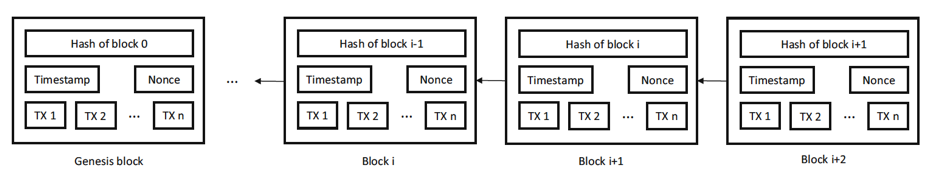
\includegraphics[width=1\textwidth]{figures/blockchain}
  \caption{Voorbeeld van een blockchain \citep{zheng2016blockchain}}
  \label{blockchain_reference}
\end{figure}

\clearpage
\subsection{Eigenschappen}

\cite{zheng2017overview}[Key Characteristics of Blockchain, p.5] stelt dat er vier eigenschappen zijn die een Blockchain definiëren:

\paragraph{Decentralisatie} In traditionele gecentraliseerde transactie systemen wordt iedere transactie gevalideerd door een centrale vertrouwde organisatie (e.g.\ banken), waardoor er een bottleneck gecreëerd wordt door de transacties te verwerken door centrale informatiesystemen. In contrast daarmee is een derde partij niet meer nodig in blockchain systemen. Consensus algoritmes zorgen ervoor dat data consistent is binnen het netwerk.

\paragraph{Persisentie} Transacties kunnen snel gevalideerd worden en invalide transacties zullen niet toegelaten worden. Het is bijna onmogelijk om te transacties verwijderen of ongedaan te maken als ze zijn opgenomen in de blockchain.

\paragraph{Anonimiteit} Elke gebruiker van het systeem kan interacteren zonder zijn ``echte" identiteit kenbaar te maken.

\paragraph{Controleerbaarheid} In bitcoin wordt de balans van een gebruiker opgeslagen door gebruik te maken van het Unspent Transaction Output (UTXO) model. Elke transactie refereert naar eerdere unspent transacties. Wanneer de huidige transactie is opgenomen in de blockchain, zal de staat van alle gerefereerde transacties verandert worden van ``unspent" naar ``spent". Hierdoor zijn transacties makkelijk te valideren en te traceren.

\newpage
\section{Toepassing}

\textit{In dit hoofdstuk wordt de vraag ``Waarvoor wordt Blockchain technologie gebruikt?'' beantwoord. Deze vraag is opgesteld omdat er geen toepassing bekend is voor de te realiseren Blockchain onderdelen, zoals aangegeven in de beschrijving van de aanpak. Het antwoord op deze vraag dient om de opdrachtgever te informeren in wat er mogelijk is met Blockchain technologie om zo een toepassing te kiezen voor het te ontwikkelen Proof of Concept. \\ \\ Er is in het bijzonder aandacht geschonken aan Blockchain als development platform aangezien de opdrachtomschrijving, bijlage \ref{appendix:opdrachtformulering}, spreekt over de realisatie van het onderdeel Smart Contract. Uitleg over het onderdeel \glspl{smart_contract} is beperkt gebleven aangezien het buiten de scope van de opdracht valt.
}

Blockchain technologie wordt steeds vaker toegepast voor het opzetten van een gedecentraliseerd systeem. Aangezien de bekendste toepassing van blockchain technologie een financieel systeem is wordt het vaak gezien als technologie die specifiek bedoeld is om financiële diensten te ondersteunen. In de literatuur wordt er echter veel geëxperimenteerd en gespeculeerd over andere mogelijke toepassingen van blockchain technologie.

\begin{wrapfigure}{r}{0.5\textwidth}
  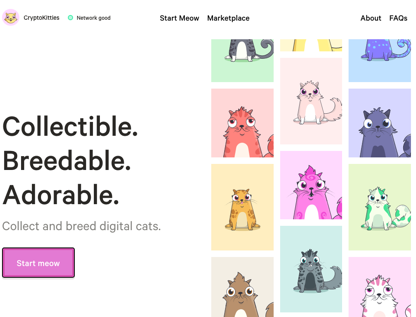
\includegraphics{figures/cryptokitties}
  \caption{CryptoKitties, een spel dat gebruik maakt van Blockchain technologie.}
  \label{cryptokitties}
\end{wrapfigure}

Zo stelt \citeauthor{atzori2015blockchain}, (\citeyear{atzori2015blockchain}) bijvoorbeeld dat blockchain technologie ingezet kan worden om de politiek en de maatschappij te veranderen. In een andere studie gedaan door \citeauthor{crosby2016blockchain}, (\citeyear{crosby2016blockchain}) wordt er onderscheid gemaakt tussen financiële en niet-financiële toepassingen die mogelijk veranderd kunnen worden door blockchain technologie. Een aantal voorbeelden die gegeven worden zijn de toepassingen bij verzekeringen, gedecentraliseerde opslag en domeinregistratie. In fig. \ref{cryptokitties} is een afbeelding te zien van de website van CryptoKitties, een van de eerste spellen die gebruik maakt van blockchain technologie, namelijk het Ethereum netwerk.

\clearpage
\subsection{Ontwikkelplatform}
Blockchains als Ethereum, EOS en HyperLedger bieden hun functionaliteit aan als development platform. Het stelt ontwikkelaars in staat om hun eigen toepassingen te realiseren, zogenaamde \gls{dapps}.

\begin{lstlisting}[
  linewidth=\textwidth, breaklines=true, 
  basicstyle=\small, label={smart_contract},
  caption={Smart contract voor ``The Greeter'' geschreven in Solidity, zoals gepresenteerd in een tutorial voor Smart Contracts op het Ethereum netwerk \citep{ethereum_smart_contract}.}]
  contract Mortal {
    /* Define variable owner of the type address */
    address owner;

    /* This function is executed at initialization and sets the owner of the contract */
    function Mortal() { owner = msg.sender; }

    /* Function to recover the funds on the contract */
    function kill() { if (msg.sender == owner) selfdestruct(owner); }
  }

  contract Greeter is Mortal {
    /* Define variable greeting of the type string */
    string greeting;

    /* This runs when the contract is executed */
    function Greeter(string _greeting) public {
        greeting = _greeting;
    }

    /* Main function */
    function greet() constant returns (string) {
        return greeting;
    }
  }
\end{lstlisting}

Door het gebruik van \glspl{smart_contract}, te zien in fig. \ref{smart_contract}, is het mogelijk om functionaliteit bij transacties te voegen om extra handelingen, die niet gerelateerd zijn tot de kern van een Blockchain implementatie, uit te voeren. Hieronder is een voorbeeld gegeven wat er mogelijk is met betrekking tot \gls{dapps}.

\paragraph{CryptoKitties} is een spel dat gebruikt maakt van het Ethereum platform, bestaand uit verzamelbare en fokbare digitale katten. De uitwisseling en het fokken van CryptoKitties wordt vastgelegd in het Ethereum netwerk door middel van \glspl{smart_contract}. Wanneer twee CryptoKitties gefokt worden, wordt het uiterlijk en de eigenschappen van hun nageslacht bepaald door het 256-bits genoom van elke ouder en een toeval element, wat leidt tot 4 miljard mogelijke genetische variaties \citep{cryptokitties}.


\newpage
\section{Architectuur}
\label{chapter:architecture}

\textit{
  In dit hoofdstuk wordt de vraag ``Uit welke componenten bestaat een Blockchain implementatie?'' behandeld. Het antwoord op deze vraag dient om een duidelijk beeld te scheppen welke componenten betrekking hebben op de onderdelen Distributed Network en Identity Management en tevens gebruikt zal worden als afstemming met zowel de opdrachtgever als de medeafstudeerder, Kevin Bos. 
}

\begin{wrapfigure}{r}{0.5\textwidth}
  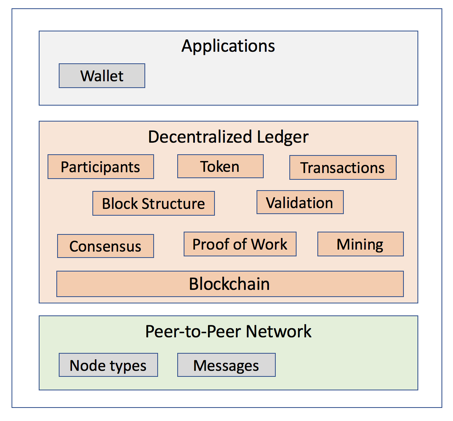
\includegraphics{figures/blockchain_architecture}
  \caption{Blockchain architectuur.}
  \label{blockchain_architecture}
\end{wrapfigure}

In fig. \ref{blockchain_architecture} is een overzicht weergegeven van de onderdelen en componenten waaruit een Blockchain bestaat. In de applicatie laag is de wallet te vinden die een gebruiker van de Blockchain doorgaans gebruikt om transacties te verrichten. De onderliggende functionaliteit van de wallet doet niets meer als het bijhouden van public- en private keys van de gebruiker waarop de nog niet uitgegeven tokens (cryptocurrency, contracten, diensten) geregistreerd staan.

De Decentralized Ledger is de kern van de technologie en zorgt ervoor dat de globale blockchain consistent en fraudebestending blijft. De fundamentele structuur achter de gehele technologie is de blockchain, waar transacties gegroepeerd worden in blokken en elk blok crypto grafisch verbonden wordt met het vorige blok. Een transactie is een vorm van uitwisseling van tokens tussen deelnemers, ook wel nodes genoemd, van het systeem. Voordat transacties als valide worden beschouwd, ondergaan ze een validatie proces die uitgevoerd wordt door alle nodes in het systeem. Het proces van het groeperen van transacties in een blok dat toegevoegd wordt aan het einde van de blockchain wordt ook wel minen genoemd. Om er zeker van te zijn dat er overeenstemming is onder alle deelnemers over welke blockchain legitiem is, wordt er gebruik gemaakt van een Proof-of-Work algoritme tijdens het mining proces om te bepalen welke ketting de meeste inspanning vereist.

Het laatste component is het peer-to-peer netwerk, waarin verschillende node types gedefinieerd zijn. Zo heb je bijvoorbeeld de validatie node die transacties valideert en een mining node die het mining process uitvoert. Om de Decentralized Ledger bij te werken en te onderhouden communiceren de nodes met elkaar door middel van het versturen van berichten.

\newpage
\section{Gedistribueerd netwerk}

\textit{
  In dit hoofdstuk wordt de vraag ``Waaruit bestaat het onderdeel gedistribueerd netwerk binnen Blockchain technologie?'' behandeld. Bij deze vraag wordt er gekeken naar de geïdentificeerde onderdelen uit hoofdstuk \ref{chapter:architecture}. Er wordt een korte introductie gegeven in peer-to-peer netwerken en waarom het een belangrijk onderdeel is bij het realiseren van de eigenschappen, behandeld in hoofdstuk \ref{chapter:blockchain}, van een Blockchain implementatie. Het antwoord op deze vraag zal helpen bij het selecteren van zoektermen die gebruikt worden om inventarisatie te doen op de onderdelen die het Distributed Network omvat.
}

Het onderdeel Distributed Network bestaat uit het verspreiden, uitbreiden en het behalen van consensus over de staat van de Blockchain tussen de deelnemers aan het netwerk. Om dit te doen wordt er gebruik gemaakt van een \acrfull{P2P} implementatie waarbij het mogelijk is om een lokale versie van de ketting aan te bieden aan andere nodes binnen het \acrshort{P2P} netwerk, om zo de huidige chain up-to-date te houden met wijzigingen die gedaan zijn door de verschillende verbonden nodes. Dit leidt tot een complex probleem dat beschreven wordt als het Byzantine Generals Problem \citep{lamport1982byzantine}, wat beschrijft aan de hand van een abstract voorbeeld dat het essentieel is voor een betrouwbaar computersysteem om te kunnen gaan met fouten die optreden in een of meer van de componenten, waardoor het kan voorkomen dat er conflicterende informatie verstuurd wordt naar de andere componenten van het systeem.

\textbf{Peer-to-Peer}

De term \acrshort{P2P} betekend dat alle computers die deel uit maken van het netwerk, peers van elkaar zijn, gelijk aan elkaar zijn, er geen speciale "nodes" zijn en dat alle deelnemers in het netwerk de last delen van het leveren van netwerkdiensten \citep[~p.171]{Antonopoulos:2014:MBU:2695500}. Het is een techniek die cruciaal is voor Blockchain en de doelen die het probeert te behalen. \acrshort{P2P} systemen verdelen namelijk de kosten om data te delen – opslag voor bestanden en bandbreedte voor het versturen van de bestanden – over de deelnemers van het netwerk, waardoor applicaties kunnen schalen zonder krachtige, dure servers \citep{bawa2003peer}.

Een van de bekendste toepassingen van een peer-to-peer netwerk is het creëren van een gedecentralizeerd file-sharing protocol. Implementaties hiervan zijn BitTorrent, LimeWire en Gnutella. Om een bestand te distribueren wordt het opgesplitst in delen, waarbij er een hash gecreëerd wordt voor elk deel. Wanneer een andere deelnemer van het netwerk een deel ontvangt wordt er gekeken aan de hand van de hash of het onderdeel geen fouten bevat. Bestanden worden geregistreerd in het netwerk door het opnemen van de hashes in een zogenaamde \textit{tracker} die gebruik maakt van een \acrfull{DHT}. Een voorbeeld van een DHT is te zien in fig. \ref{DHT}.

\newpage
\begin{wrapfigure}{l}{0.6\textwidth}
  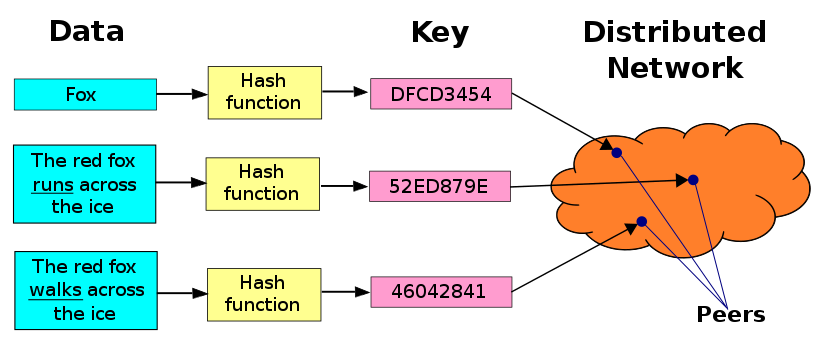
\includegraphics[width=0.6\textwidth]{figures/DHT}
  \caption[Distributed Hash Table] {
    Door het vertalen van data naar een cryptografische sleutel is het mogelijk om aan de hand van de sleutel de data op te vragen aan peers die de data bezitten.
  }
  \label{DHT}
\end{wrapfigure}

\textbf{Consensus}

Consensus is een dynamische manier van het behalen van overeenstemming in een groep. In blockchain implementaties wordt het gebruikt om overeenstemming te behalen over de staat van het netwerk en de volgorde waarin transacties gedaan zijn. Met het consensus algoritme wordt er een zekere mate van veiligheid gewaarborgd, waardoor het voor een kwaadwillende deelnemer (bijna) onmogelijk dient te zijn om het netwerk te beïnvloeden. Het kan voorkomen dat een kwaadwillende deelnemer probeert het netwerk te beïnvloeden waardoor er tegenstrijdige consensus kan optreden en een \gls{fork} ontstaat in het netwerk.

\textbf{Fork}

Een \gls{fork} is een splitsing in het netwerk die veroorzaakt is door een verandering in het protocol of door het toedoen van kwaadwillende deelnemer(s). Er zijn hiervoor twee categorieën \glspl{fork}, een \gls{hard_fork} en een \gls{soft_fork}.

\paragraph{Soft fork}

is een verandering in het netwerk die terugwaartse compatibiliteit heeft met eerdere versies van het protocol. Als voorbeeld kan er voor gekozen worden dat in plaats van blocks een limiet hebben van 1MB, de regel aangepast wordt zodat blocks een grootte van 500K moeten hebben. Als een \gls{soft_fork} verkeerd gaat is het nog steeds mogelijk dat er een \gls{hard_fork} optreed \citep[Soft Fork]{coindesk:forks}.

\paragraph{Hard fork}

is een protocol update waarbij een nieuwe regel geïntroduceerd wordt, waardoor het netwerk geen compatibiliteit heeft met oudere versies. Dit zorgt ervoor dat deelnemers in het netwerk die een oudere versie hebben, de nieuwe transacties als invalide beschouwen. Een voorbeeld van een regel waarbij een \gls{hard_fork} ontstaat is bijvoorbeeld het ophogen van de block grootte naar 2MB in plaats van 1MB \citep[Hard Fork]{coindesk:forks}. 

\newpage
\textbf{\Glspl{node}}

Alhoewel de structuur van een Blockchain dezelfde structuur afdwingt voor de \glspl{node} in het netwerk, kunnen zij een verschillende rol spelen. Alle \glspl{node} binnen het netwerk valideren, verspreiden en ontdekken en onderhouden connecties met andere \glspl{node} binnen het netwerk. In fig. \ref{blockchain_node_types} is te zien welke services een  \gls{full_node} in het Bitcoin netwerk aanbiedt. 

\begin{wrapfigure}{r}{0.4\textwidth}
  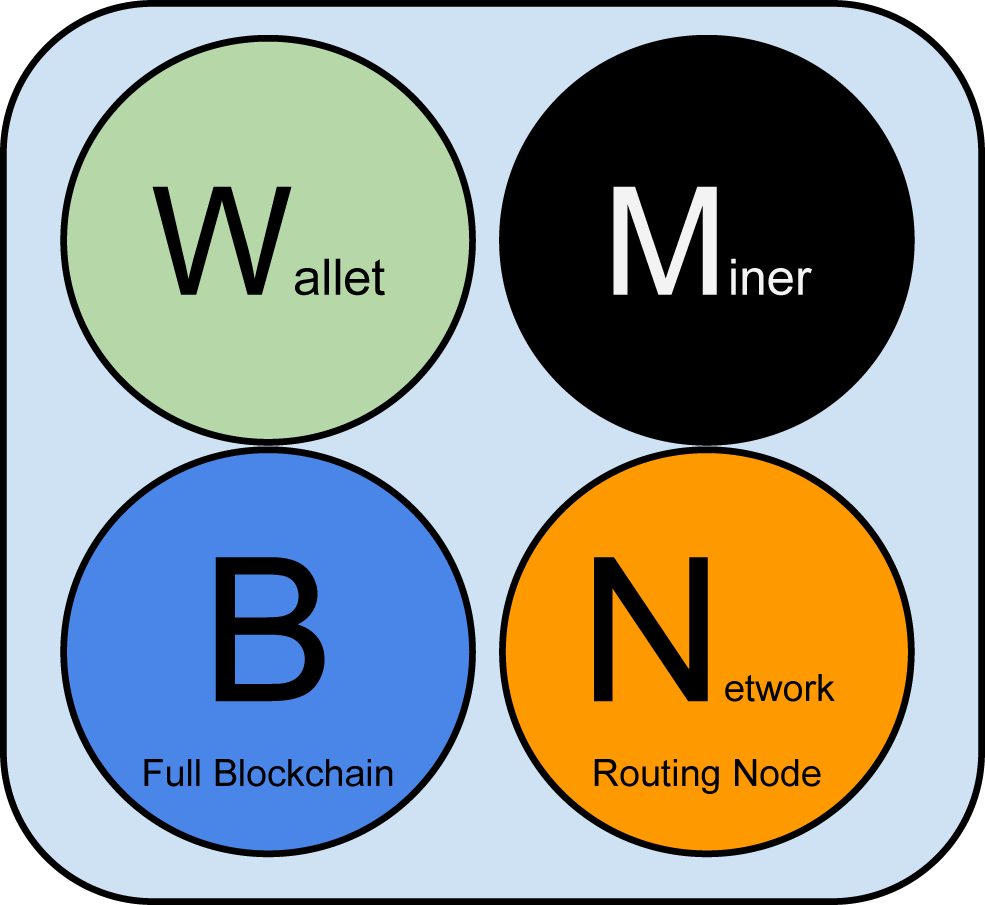
\includegraphics[width=0.4\textwidth]{figures/bitcoin_node_types}
  \caption[Bitcoin Node functionaliteiten] {
    Een bitcoin netwerk node die alle functies bevat: wallet, mining, blockchain database en netwerk routing, \citep[p.~172]{Antonopoulos:2014:MBU:2695500}.
  }
  \label{blockchain_node_types}
\end{wrapfigure}

Een \textbf{\gls{full_node}} is een collectie van functies, namelijk routing, de blockchain database, het mining proces en wallet services en bevat een gehele kopie van de actuele blockchain. Een \textbf{\gls{wallet_node}} is een deelnemer in het netwerk die een subset van de gehele blockchain bevat om transacties te versturen, verifiëren en ontvangen. De \textbf{\glspl{mining_node}} concurreren voor het creëren van een nieuw block door het uitvoeren van het Proof-of-Work algoritme. 

Alle \glspl{node} binnen het netwerk bieden gelijke diensten aan en kunnen gebruik maken van dezelfde diensten terwijl ze samenwerken door middel van een consensus protocol.

De verschillende services binnen het netwerk en de \gls{node} types die hieraan meewerken is dan ook een architecturale keuze over de indeling van het \acrshort{P2P} netwerk.


\newpage
\section{Identiteit}

\textit{
  In dit hoofdstuk wordt de vraag ``Waaruit bestaat het onderdeel Identity Management binnen Blockchain technologie?'' behandeld. Zoals beschreven in hoofdstuk \ref{chapter:blockchain} zijn anonimiteit en controleerbaarheid belangrijke eigenschappen van een Blockchain implementatie. Allereerst zal er beschreven worden wat identiteit inhoud binnen een Blockchain en welke mogelijke vormen van management er zijn. Het antwoord op deze vraag wordt gebruikt om zoektermen op te stellen en een afbakening te creëren voor de te onderzoeken protocollen.
}

In het vooronderzoek is er weinig gevonden over Identity Management en zelf wist ik dan ook niet goed wat dit onderdeel voor functionaliteiten bevat. In eerste instantie is er gekeken naar de verschillende types van Blockchain, waarbij gebruikers van het systeem autorisatie hebben tot bepaalde acties. Om een beter beeld te schetsen en de afbakening van het onderdeel compleet te maken voor het onderzoek is er besloten om een gesprek te houden met Pim Otte.

Uit dit gesprek is naar voren gekomen dat het Identity Management gedeelte gaat over hoe de Blockchain implementatie met public keys (de identiteit van een gebruiker) omgaat. Als tip werd er gegeven om te kijken naar de wallet software indien beschikbaar. Dit is software die de public- en private key beheert voor een gebruiker. Daarnaast is er ook een tip gegeven over het onderdeel Distributed Network. Om een goed beeld te krijgen van de aanvallen waar het netwerk tegen bestand is, is het handig om een threat model op te stellen.

Het onderdeel Identity Management beschrijft hoe de Blockchain omgaat met de identiteit van gebruiker die deel uitmaakt van het netwerk. Daarnaast is het mogelijk dat een bepaald type Blockchain meer doet dan alleen de identiteit van de gebruiker beheerd of maskeert. 

\subsection{Categorieën}

\cite{zheng2017overview} deelt Blockchain implementaties op in drie categorieën, waarin de zichtbaarheid en participatie in het consensus proces gelimiteerd.

\paragraph{Public} In een public Blockchain zijn alle transacties publiekelijk inzichtbaar en iedereen in het netwerk maakt onderdeel uit van het consensus proces. Dit wordt ook wel gezien als een permissionless Blockchain.

\paragraph{Consortium} In een consortium Blockchain is er een groep van vooraf geselecteerde nodes die deel uitmaken van het consensus proces. De consortium Blockchain wordt meestal gebruikt door meerdere organisaties en is gedeeltelijk gedecentraliseerd. Omdat bepaalde nodes geïdentificeerd dienen te worden wordt dit type Blockchain gezien als een permissioned Blockchain.

\clearpage
\paragraph{Private} In een private Blockchain worden alleen nodes van een specifieke organisatie toegelaten tot het consensus proces. Het wordt ook wel als een centraal netwerk gezien omdat het in volledige controle is van één organisatie. Omdat het hier gaat om volledige restrictie tot het Blockchain netwerk wordt dit type Blockchain gezien als een permissioned Blockchain.

In een consortium en een private Blockchain dient de gebruiker zich te identificeren aan de hand van een identiteit. Zoals eerder vermeld maakt Blockchain gebruik van een public- en private keys om de gebruiker te identificeren. Dit hanteert in zekere mate een permissie model waarbij de autorisatie van een gebruiker vastgelegd word aan de hand van de identificatie (i.e.\ de public key) die het netwerk gebruikt.

\subsection{Identificatie}

Identificatie wordt doorgaans gedaan aan de hand van een public key van een gebruiker. Een van de missies van Blockchain is totale anonimiteit, alleen zijn er een aantal problemen die volledige anonimiteit tegengaan. Om de terminologie duidelijk te maken wordt hieronder het verschil tussen pseudoniem en anoniem uitgelegd aan de hand van voorbeelden vanuit het Bitcoin protocol.

\begin{formal}
  ``Anonymity is the state of being not identifiable within a set of subjects, the anonymity set."
  \\ \cite{pfitzmann2001anonymity}.
\end{formal}

\paragraph{Pseudoniem} 

Bij een pseudoniem gaat er om een referentie naar de identiteit. 

\paragraph{Anoniem}







\newpage
\section{Obstakels}

In het vooronderzoek is er weinig gevonden over Identity Management en zelf wist ik dan ook niet goed wat dit onderdeel voor functionaliteiten bevat. In eerste instantie is er gekeken naar de verschillende types van Blockchain, waarbij gebruikers van het systeem autorisatie hebben tot bepaalde acties. Om een beter beeld te schetsen en de afbakening van het onderdeel compleet te maken voor het onderzoek is er besloten om een gesprek te houden met de Blockchain Expert.

Uit dit gesprek is naar voren gekomen dat het Identity Management gedeelte gaat over hoe de Blockchain implementatie met public keys (de identiteit van een gebruiker) omgaat. Als tip werd er gegeven om te kijken naar de wallet software indien beschikbaar. Dit is software die de public- en private key beheert voor een gebruiker. Daarnaast is er ook een tip gegeven over het onderdeel Distributed Network. Om een goed beeld te krijgen van de aanvallen waar het netwerk tegen bestand is, is het handig om een threat model op te stellen.
\section{Conclusie}

Naar aanleiding van de resultaten uit het vooronderzoek zijn er keuzes gemaakt die zich reflecteren in het onderzoek. Hieronder is per vraag beschreven over de implicaties die de resultaten gaven tegenover het onderzoek. 

Uit de vraag ``Waaruit bestaat het onderdeel Distributed Network binnen Blockchain technologie?'' is gebleken dat het consensus proces invloed heeft op de structuur van het netwerk. Het soort consensus zal dan ook gebruikt worden om de verschillende type Distributed Networks te onderscheiden. Ook zullen de verschillende type van nodes onderzocht worden om te identificeren welke bijdrage een bepaald type node levert om het netwerk in stand te houden. 

In de resultaten van de vraag ``Waaruit bestaat het onderdeel Identity Management binnen Blockchain technologie?'' is er geïdentificeerd dat er twee manieren zijn waarop de privacy van de gebruiker gewaarborgd wordt, namelijk of het een permissionless of permissioned Blockchain is en de identificatie van de gebruiker binnen het netwerk. Er wordt aangegeven dat het niveau van privacy en autorisatie ligt aan de categorie van waar de Blockchain deel van uitmaakt.

\begin{enumerate}[noitemsep]
  \item Zichtbaarheid van acties die de gebruiker onderneemt op de Blockchain.
  \item Autorisaties voor acties die de gebruiker wilt ondernemen op de Blockchain.
\end{enumerate}


  \chapter{Selectie protocollen}
\label{selectie}

Om het onderzoek binnen de beschikbare tijd te houden is er in overleg met de Blockchain Expert voor gekozen om een initiële selectie van de top 20 verhandelde cryptocurrencies te bekijken, waarna er een selectie van vier implementaties gemaakt wordt gebaseerd op de beschikbare informatie, het type consensus en hoe het omgaat met de identiteit van de gebruiker. Deze vier implementaties zullen vervolgens uitvoerig onderzocht en beschreven worden op de werking van de onderdelen Distributed Network en Identity Management. 

\section{Coinmarketcap}

De selectie van de top 20 verhandelde cryptocurrencies wordt gedaan aan de hand van de website \href{https://coinmarketcap.com/}{Coinmarketcap}. Hierop zijn meerdere overzichten te zien die te maken hebben met de handelsvolume van cryptocurrencies.
\begin{wrapfigure}[17]{r}{0.6\textwidth}
  \begin{center}
    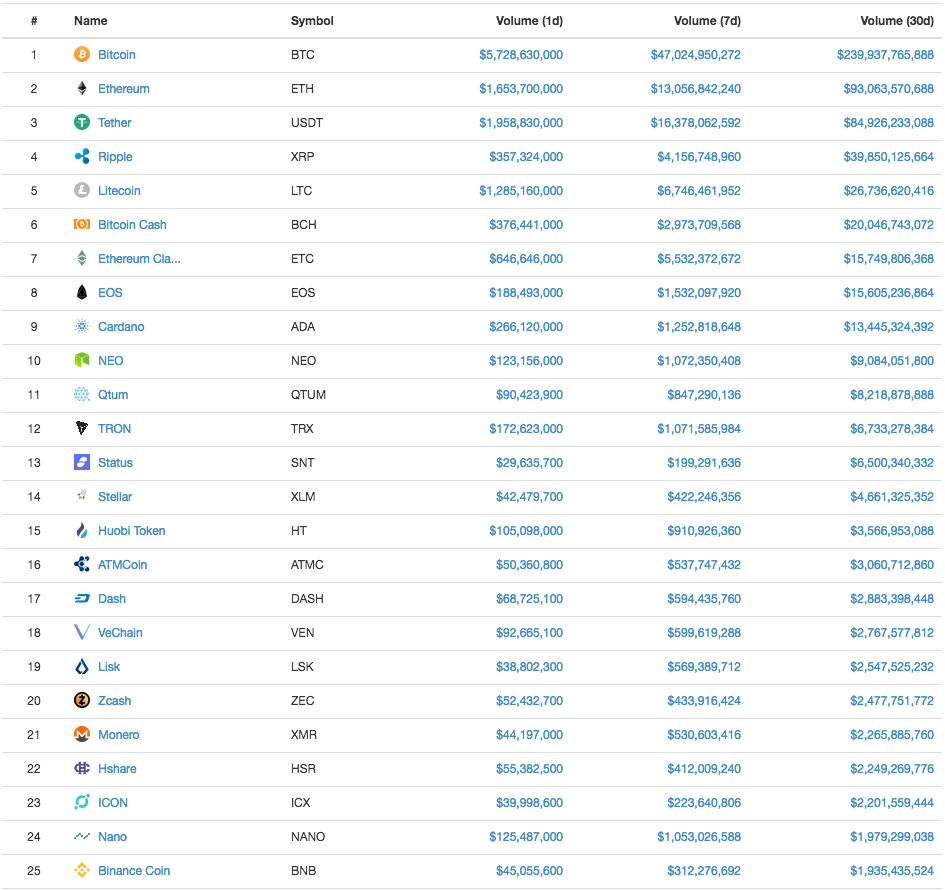
\includegraphics[width=0.6\textwidth]{figures/coinmarketcap}
    \caption[Snapshot Coinmarketcap] {
      Meest verhandelde cryptocurrencies in de maand februari zoals gepresenteerd op de website van Coinmarketcap.
    }
    \label{coinmarketcap}
  \end{center}
\end{wrapfigure}
Een van de overzichten is het maandelijkse handelsvolume zoals te zien in fig. \ref{coinmarketcap}. Deze lijst is gebruikt voor het selecteren van de initiële top 20 van cryptocurrencies. Door de architecturen achter de meest verhandelde cryptocurrencies te gebruiken wordt ervoor gezorgd dat er robuuste en volwassen implementaties bekeken worden.

\subsubsection{Hard forks}
Om te voorkomen dat er soortgelijke implementaties bekeken worden is ervoor gekozen om de hard forks niet mee te nemen in de initiële selectie. Een voorbeeld hiervan is Bitcoin Cash ten opzichte van Bitcoin. Alhoewel Bitcoin Cash een aantal veranderingen doorgemaakt heeft sinds de afsplitsing van het Bitcoin protocol, wordt het niet meegenomen omdat er in zekere mate overeenkomsten aanwezig zijn.

\section{Attributen}
Om een selectie te maken tussen de top 20 verhandelde cryptocurrencies is er gekeken naar attributen die nader beschreven zijn in onderstaand tabel.

\begin{centering}
  \begin{table}[ht]
    \label{selectie-attributen}
    \caption{Attributen opgesteld voor initiële selectie implementaties.}
    \makebox[\textwidth]{%
      \begin{tabular}{r|p{10cm}}
        \textbf{Identity Management} & Of de implementatie actief iets onderneemt dat te maken heeft met Identity Management, e.g.\ het vergroten van de privacy van de gebruiker. \\
        \hline
        \textbf{Whitepaper} & Of de implementatie een technische whitepaper beschikbaar heeft. \\
        \hline
        \textbf{Open-source} & Of er een referentie implementatie open-source beschikbaar is voor het bestuderen van de code. \\
        \hline
        \textbf{In circulatie sinds} & Een indicatie van de volwassenheid van de implementatie. \\ 
        \hline
        \textbf{DApps platform} & Of het gebruikt kan worden als development platform. Hierbij zal er een zekere mate van modulariteit nodig zijn in de broncode. \\ 
        \hline
        \textbf{Consensus} & Welk consensus algoritme gebruikt wordt. Dit is van invloed op de werking van het onderdeel Distributed Network. \\
      \end{tabular}
    }
  \end{table}
\end{centering}

Het doel van de attributen is een indicatie te krijgen over de hoeveelheid documentatie die een implementatie beschikbaar heeft. Dit is dan ook de doorslaggevende factor geweest bij het selecteren van vier implementaties die nader onderzocht zullen worden.

\newpage
\subsubsection{Totstandkoming}

Hieronder wordt kort beschreven hoe de inventarisatie van de attributen gedaan is.

\paragraph{Identity Management}
Om vast te stellen of een implementatie iets onderneemt in de vorm van Identity Management wordt er gebruik gemaakt van bestaande literatuur over de implementatie. Door middel van het scannend lezen van de beschikbare literatuur wordt er vastgesteld of er beschrijvingen zijn van de identiteit binnen de Blockchain implementatie en hoe dit tot stand is gekomen.

\paragraph{Whitepaper}
Bijna elke Blockchain implementatie heeft een website waarin de functionaliteiten gepresenteerd worden voor de mogelijke gebruiker. Om erachter te komen of er een whitepaper beschikbaar is, is een scan van de website voldoende.

\paragraph{Open-source}
Om na te gaan of een implementatie open-source is wordt er gezocht op Github en Bitbucket op de aanwezigheid van de organisatie en/of protocol naam.

\paragraph{In circulatie sinds}

Om de circulatiedatum te achterhalen is gebruik gemaakt van Wikipedia. Hierbij is een schatting van de datum waarop de Blockchain implementatie actief is geworden al voldoende.

\paragraph{DApps platform}

Om na te gaan of de implementatie de ontwikkeling van gedistribueerde applicaties ondersteund is er gezocht naar development tutorials op de websites van de Blockchain implementatie.

\paragraph{Consensus}

Het type consensus dat gebruikt wordt is tevens te achterhalen uit de besschikbare documentatie en wordt achterhaald door scannend te lezen.

\newpage
\section{Selectie}

Aan de hand van deze attributen is een lijst opgesteld, te zien in tabel \ref{bijlage_selectie_implementatie}, waarin de initiële selectie te vinden is met bijbehorende attributen van de implementatie. Over sommige implementaties zoals VeChain is weinig informatie gevonden waardoor ze direct afvallen. Aan de hand van deze attributen zijn de volgende protocollen geselecteerd.

\paragraph{Cardano} is een Blockchain protocol waarin onderzoek centraal staat. Het beweert dan ook het eerste blockchain platform te zijn die ontstaan is uit een filosofisch en onderzoek gedreven aanpak. De implementatie van het protocol is volledig open-source en er is een technische whitepaper beschikbaar. Daarnaast is er ook een platform om je eigen applicaties op het netwerk te creëren.

\paragraph{Monero} is een implementatie die beweert dat de gebruiker volledig ontraceerbaar is. Het is net zoals Cardano een volledige open-source implementatie en maakt gebruik van egalitair Proof of Work. Daarnaast heeft het protocol een technische whitepaper. 

\paragraph{Bitcoin} is het originele protocol waarin de Blockchain technologie gerealiseerd is. Door de grote hoeveelheid onderzoek die gedaan is naar Bitcoin is er een overvloed van informatie, waarin niet alleen informatie over Bitcoin gegeven wordt maar ook over het Blockchain domein. De implementatie van het protocol is wederom volledig open-source en er is een technische whitepaper beschikbaar.

\paragraph{EOS} is een relatief nieuw protocol die zojuist een test netwerk gelanceerd heeft. Ook deze implementatie is beschreven in een whitepaper, is volledig open-source en kan gebruikt worden als platform om applicaties op te ontwikkelen. Consensus binnen het protocol wordt bereikt door Delegated Proof of Stake.

  \chapter{Onderzoek}
\textit{In dit hoofdstuk worden de werkzaamheden met betrekking tot het uitvoeren van het onderzoek beschreven. De aanleiding voor het onderzoek is te vinden in hoofdstuk \ref{Aanpak}, waarin wordt beschreven waarom dit onderzoek meerwaarde heeft binnen de opdracht.}

Het onderzoek dient voor het opstellen van het adviesrapport waarin protocollen worden  gepresenteerd  aan Quintor die mogelijk geïmplementeerd kunnen worden tijdens de realisatie van het Proof-of-Concept. Het betreft exploratief onderzoek waarin case-study gebruikt wordt om een gedetailleerde omschrijving van de onderdelen Identity Management en Distributed Network op te stellen van Blockchain implementaties die geselecteerd zijn in hoofdstuk \ref{selectie}. De kennis die hiermee wordt opgebouwd kan eventueel gebruikt worden in vervolgonderzoek.

In het onderzoek staat de onderstaande hoofdvraag centraal:
\begin{formal}
  Welke protocol implementaties kunnen toegepast worden om de onderdelen Distributed Network en Identity Management te realiseren voor een Blockchain implementatie?
\end{formal}

Omdat de hoofdvraag te groot is om in een keer te beantwoorden is het opgesplitst in de volgende deelvragen:

\begin{enumerate}[noitemsep]
  \item "Welke soorten gedistribueerde netwerken worden er gebruikt?"
  \item "Hoe werken de gedistribueerde netwerken en tegen welke gevaren zijn ze bestendig?"
  \item "Hoe wordt er omgegaan met de identiteit van de gebruiker?
\end{enumerate}

Op de volgende pagina's is per deelvraag behandeld wat de bijdrage van het antwoord oplevert aan de doelstelling, hoe de vraag beantwoord is en wordt er concreet de bevindingen besproken.

\clearpage
\section{Opzet}

Om te achterhalen welke protocol implementaties toegepast kunnen worden om de onderdelen Distributed Network en Identity Management te realiseren voer ik kwalitatief, exploratief onderzoek uit. Door het uitgevoerde vooronderzoek heb ik wel basiskennis over de onderdelen, maar weet ik nog niet de details. Om die reden heb ik er dan ook voor gekozen om het exploratief aan te pakken. Het gevaar hierbij is dat er teveel informatie geanalyseerd wordt waardoor het onderzoek te uitgebreid wordt.

\subsection{Dataverzameling}

De benodigde data zal ik verzamelen door het uitvoeren van deskresearch, waarbij ik de geselecteerde Blockchain protocol implementaties zal analyseren. De data die ik hiervoor nodig hebt komt vooral uit de whitepapers die beschikbaar zijn voor elke implementatie. Daarnaast worden er zo veel mogelijk academische bronnen gebruikt. Om deze, mogelijk aanvullende, academische bronnen te vinden zal ik gebruik maken van het schoolportaal en Google Scholar. Hierbij zal er gelet worden op de kwaliteit van de studie, door te achterhalen of het gebruikt wordt in andere studies en te kijken of het peer reviewed is.

\subsection{Dataomschrijving}

De Blockchain implementaties zullen in eerste instantie geselecteerd worden op de aanwezigheid van het onderdeel Identity Management. Hierbij zal ik kijken of de implementatie actief iets onderneemt voor bijvoorbeeld het verhogen van de privacy van de gebruiker. Daarnaast zal er gekeken worden naar de beschikbare hoeveelheid informatie.

\subsection{Analysemethode}

De methode die ik zal gebruiken voor het analyseren van de data is het uitvoeren van cumulatieve case-studies. Hierbij zullen er meerdere bronnen bekeken worden van een Blockchain implementatie waarna een aggregatie gemaakt wordt van de benodigde data voor het beantwoorden van de opgestelde vragen.

\newpage
\section{Soorten netwerken}

\textit{In dit hoofdstuk wordt de vraag ``Welke soorten gedistribueerde netwerken worden er gebruikt?'' behandeld. Het doel van de vraag is om de architectuurkeuzes op het gebied van het Distributed Network onderdeel op te stellen, en waar mogelijk is de implicaties van de keuze tegenover het Identity Management onderdeel.}

% In het vooronderzoek is er gevonden dat het consensusproces van grote invloed kan zijn op de architectuurkeuzes van het gedistribueerd netwerk. Er is dan ook voor gekozen om in het onderzoek het netwerksoort synoniem te stellen aan het type consensus die de implementatie gebruikt.

\subsection{Aanpak}

\begin{wrapfigure}[14]{r}{0.5\textwidth}
  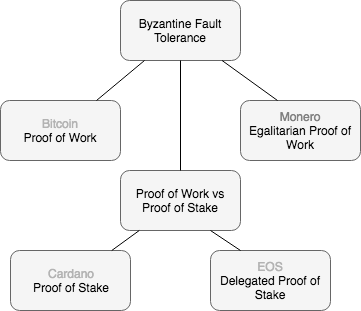
\includegraphics[width=0.5\textwidth]{figures/uitwerking_soorten}
  \caption[Opbouw beantwoording ``Soorten netwerken'']{Termen die als leidraad gebruikt zijn om het resultaat te beschrijven}
  \label{opbouw:netwerken}
\end{wrapfigure}

In fig. \ref{opbouw:netwerken} is te zien welke (globale) termen er gebruikt zijn om de benodigde informatie te vinden. In de meeste gevallen is de beschikbare whitepaper van de implementatie voldoende geweest om de werking van het consensus te beschrijven. Hieronder is de werkwijze en denkwijze uitgeschreven per individueel onderdeel.

\subsubsection{Byzantine Fault Tolerance}
Om deze vraag te beantwoorden is allereerst gezocht naar achtergrondinformatie over consensus en wat het doel ervan is. In het vooronderzoek is er informatie gevonden over het Byzantine Generals Problem \citep{lamport1982byzantine}, waarin, vertaald naar de IT-wereld, wordt gesteld dat het essentieel is voor een betrouwbaar computersysteem om te gaan met fouten in de componenten, waardoor het kan voorkomen dat er conflicterende informatie verstuurd wordt naar de andere componenten van het systeem. 

\subsubsection{Proof of Work}
Hierna zijn bij de implementaties de manier waarop consensus behaald wordt onderzocht. Voor het beschrijven van het Proof of Work algoritme is er gebruik gemaakt van de originele presentatie van het Bitcoin protocol door \cite{nakamoto2008bitcoin}, hierin was alle informatie te vinden die benodigd was. Het egalitarian Proof of Work zoals in gebruik bij Monero is beschreven in \cite{van2013cryptonote} waarin de verschillen en tekortkomingen van het Proof of Work zoals in gebruik bij Bitcoin uiteengezet wordt.

\newpage
\subsubsection{Proof of Stake}
Om een indicatie te geven van de grootste tekortkomingen op het gebied van Proof of Work en redenenen waarom Blockchain implementaties kiezen voor het implementeren van Proof of Stake is er gebruik gemaakt van de whitepaper van Cardano \cite{kiayias2017ouroboros}, waarin de gemotiveerd wordt waarom er voor Proof of Stake is gekozen in plaats van Proof of Work. Naar aanleiding van de primaire reden, namelijk dat Proof of Work enorm veel stroom verspilt, is er gezocht naar een studie die deze claim kan bevestigen, waarbij de studie van \cite{ODwyer:Bitcoin} gebruikt is om dit te bevestigen.

Bij het beschrijven van Delegated Proof of Stake zoals in gebruik bij EOS, bleek de whitepaper niet voldoende informatie te bevatten om het functioneel te beschrijven. Hiervoor is er dan ook een artikel gebruikt dat geschreven is door \cite{steemit:eos_dpos}, waarin het algoritme uitgelegd wordt.

\subsection{Conclusie}

Een gedistribueerd netwerk binnen Blockchain is getypeerd aan het consensus protocol dat gebruikt wordt. In het onderzoek zijn er twee primaire soorten geïdentificeerd, netwerken die gebruik maken van Proof of Stake of van Proof of Work, waarbij Proof of Work gebruik maakt van de rekenkracht van een \gls{node} en Proof of Stake gebruik maakt van de \gls{stake} van een \gls{node}.

\newpage
\section{Functionaliteit en gevaren}

\textit{In dit hoofdstuk wordt de vraag ``Hoe werken de gedistribueerde netwerken en tegen welke gevaren zijn ze bestendig?'' behandeld. Het doel van de vraag is om de werking van het gedistribueerd netwerk in kaart te brengen en tegenmaatregelen tegen aanvallen die in de functionaliteit verwerkt zitten te beschrijven.}

Deze vraag is opgesteld naar aanleiding van de criteria ``het moet resistant zijn tegen aanvallen'' die gesteld is in de opdrachtformulering zoals gegeven door Quintor, in te zien in bijlage \ref{appendix:opdrachtformulering}. Het eerste idee om deze vraag te beantwoorden was om een vergelijking te maken tussen de implementaties op het gebied van veiligheid, waarbij er onderzocht zou worden of een aanval op de implementatie uitgevoerd was. Dit zou uiteindelijk een ``beste'' implementatie opleveren die geadviseerd zou worden in het adviesrapport. Uiteindelijk is dit idee niet gebruikt omdat er een aantal redenenen zijn waarom dit niet zou werken:

\begin{itemize}
  \item \textbf{Protocol volwassenheid}
  \\ Het Bitcoin protocol bestaat al sinds 2011, terwijl het Monero protocol sinds 2014 bestaat. In het begin heeft Bitcoin waarschijnlijk veel te verduren gehad qua aanvallen, waardoor het via bovenstaande vergelijking slecht uit zou komen. Daarentegen heeft Monero gedurende de drie jaar zowel verbeteringen als lessen getrokken uit het Bitcoin protocol.

  \item \textbf{Adoptie van de technologie}
  \\ Proof of Work implementaties zijn vatbaar voor een \gls{majority_attack}, waarbij een gebruiker 51\% van de rekenkracht binnen het netwerk in handen moeten hebben om transacties in de Blockchain te registreren zonder dat er validatie te pas komt. Hoe minder gebruikers, hoe minder de benodigde rekenkracht om dit uit te voeren.
\end{itemize}

Om deze reden is er besloten om met de Blockchain expert over de aanpak en uiteindelijke doel van deze vraag te discussiëren, wat ertoe heeft geleid dat de focus van de vraag veranderd is van een vergelijking doen op basis van de veiligheid, het een meer beschrijvende vorm heeft gekregen waar er gekeken wordt naar componenten van het netwerk: discovery protocol, hoe informatie verstuurd wordt tussen twee \glspl{node} en wanneer mogelijk de knelpunten met betrekking tot aanvallen binnen deze componenten.

\newpage
\subsection{Aanpak}

\begin{wrapfigure}[14]{r}{0.6\textwidth}
  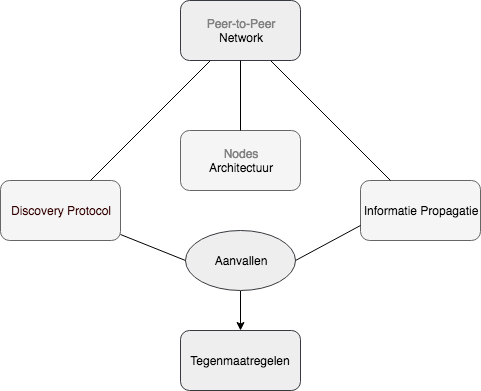
\includegraphics[width=0.6\textwidth]{figures/uitwerking_functionaliteit}
  \caption[Opbouw beantwoording ``Functionaliteit en gevaren'']{Componenten en termen die als leidraad gebruikt zijn om het resultaat te beschrijven.}
  \label{opbouw:functionaliteit}
\end{wrapfigure}

In fig. \ref{opbouw:netwerken} is te zien welke componenten er gebruikt zijn om de benodigde informatie te vinden. Hieronder is de werkwijze en denkwijze uitgeschreven per individueel onderdeel.

\subsubsection{Aanvallen}

Allereerst is er begonnen met het zoeken naar de verschillende aanvallen die mogelijk zijn op Blockchain implementaties. Binnen het gesprek met de Blockchain Expert is hierbij het woord threat model gevallen, en zijn er een aantal aanvallen aan bod gekomen:

\begin{itemize}
  \item \textbf{Eclipse attack}
  \\ Meer informatie en de definitie van een eclipse attack is gevonden in de studie van \cite{heilman2015eclipse}.

  \item \textbf{Majority attack}
  \\ De majority attack staat beschreven op de wiki van Bitcoin, waarbij er uitgelegd wordt wat het is, wat er mee mogelijk is en waarom het bijna niet uit te voeren is.

  \item \textbf{Denial of Service}
  \\ Bij Denial of Service gaat het om meerdere manieren om de uitvoering van processen binnen het netwerk te verstoren, waardoor er niet een specifieke bron te vinden is voor alle mogelijke aanvallen.

  \item \textbf{Sybil attack}
  \\ Voor het beschrijven van de sybil attack in relatie tot Blockchain is er gebruik gemaakt van de studie gedaan door \cite{conti2017survey}.

  \item \textbf{Double spending}
  \\ Informatie double spending is gevonden in de studie van \cite{karame2012double}.
\end{itemize}

Een van de knelpunten bij het beschrijven van een aanval was een studie vinden die aantoonde wat het gevolg ervan was binnen een Blockchain implementatie.

\subsubsection{Network}

Voor het beschrijven van de verschillende netwerken is er gebruikt gemaakt van niet wetenschappelijke bronnen zoals wiki's of blogs. De reden hiervoor is dat een whitepaper van een Blockchain implementatie zelden de architectuur van het netwerk beschrijft. Deze informatie is dan ook gebruikt om de verschillende componenten van het netwerk te beschrijven.

\subsection{Conclusie}

\paragraph{Bitoin} Het netwerk van Bitcoin communiceert via TCP/IP en maakt gebruik van bootstrap nodes waarmee connectie wordt gemaakt op het moment dat een nieuwe deelnemer het netwerk wilt toetreden. Informatie wordt verstuurd door een voorafgedefinieerde set aan berichttypes: \textit{inv}, \textit{tx}, \textit{block}, \textit{getdata}, waarbij een \textit{inv} bericht gebruikt wordt ter inventarisatie over de beschikbaarheid van data, \textit{tx} bericht om een transactie te versturen, \textit{block} bericht om een block te versturen, \textit{getdata} bericht om data op te vragen. \\ \\ Op het Bitcoin netwerk zijn meerdere aanvallen in de loop der jaren uitgevoerd en geïdentificeerd, een studie uit 2015 gedaan door \cite{heilman2015eclipse} toont aan dat het Peer Discovery mechanisme vatbaar is voor een Sybil Attack. \cite{nakamoto2008bitcoin} stelt dat de voordelen van het uitvoeren van een majority attack niet opweegt tegen de kosten voor de benodigde hardware om de rekenkracht te behalen. \cite{eyal2014majority} beschrijft dat het niet nodig is om een merendeel van de rekenkracht te bezitten en introduceert de aanval \gls{selfish_mining}.

\newpage
\paragraph{Cardano} Het netwerk van Cardano communiceert via TCP/IP en maakt gebruik van het Kademlia protocol waardoor het maar nodig is om één bootstrap node te gebruiken om het netwerk toe te treden. De achterliggende structuur van Kademlia is een Binary Tree waarbij de positie van een deelnemer in de Binary Tree bepaald wordt door een unieke prefix van de identificatiecode. Het protocol garandeert dat een deelnemer in verbinding staat met ten minste één andere deelnemer. Informatie wordt uitgewisseld door drie abstracte berichttypes: \textit{inv}, \textit{req}, en \textit{data}. Het \textit{inv} bericht wordt gebruikt om aan te geven dat er data beschikbaar is, het \textit{req} bericht wordt gebruikt om beschikbare data op te vragen en het \textit{data} bericht wordt vervolgens gebruikt om de data te versturen. \\ \\ Implementaties die gebruik maken van \acrshort{PoS} zijn afhankelijk van de manier waarop een leiderschapsverkiezing wordt gesimuleerd, waarbij er grote kans is dat het gevoelig is voor beïnvloedingen van kwaadwillende deelnemers in het netwerk in de vorm van een Sybil Attack. Cardano heeft een zwak punt in het Kademlia netwerk geïdentificeerd waardoor het mogelijk zou zijn om Eclipse Attack uit te voeren.

\paragraph{Monero} Het netwerk van Monero maakt gebruik van het \acrfull{I2P} protocol, dat zowel UDP/IP als TCP/IP ondersteund. Om het netwerk toe te treden wordt er gebruik gemaakt van bootstrap nodes die vastgelegd zijn in de broncode. Communicatie wordt gedaan door middel van \Glspl{tunnel}, waarbij elke deelnemer twee \Glspl{tunnel}, een inkomende en een uitgaande, heeft voor elke connectie.

\paragraph{EOS} \textit{Ten tijde van het onderzoek is er geen technische beschrijving beschikbaar over het netwerk component van EOS.}






\newpage
\section{Identiteit}

\textit{In dit hoofdstuk wordt de vraag ``Hoe wordt er omgegaan met de identiteit van de gebruiker binnen de implementatie?'' behandeld. Het doel van de vraag is om de mogelijkheden en toepassingen van identiteit te beschrijven aan de hand van de geselecteerde implementaties.}

\begin{figure}[h]
  \centering
  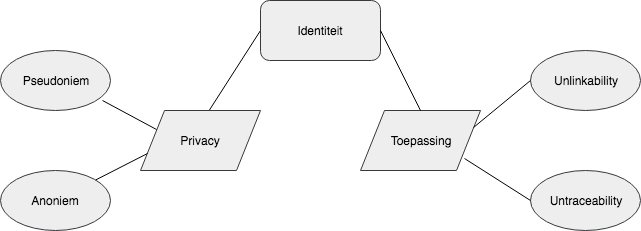
\includegraphics[width=0.8\textwidth]{figures/uitwerking_identity}
  \caption[Opbouw beantwoording ``Identiteit'']{Termen die als leidraad gebruikt zijn om het resultaat te beschrijven}
  \label{opbouw:identiteit}
\end{figure}

\subsection{Aanpak}

In fig. \ref{opbouw:identiteit} is te zien welke componenten er gebruikt zijn om de benodigde informatie te vinden. In het vooronderzoek is er gevonden dat identiteit eigenlijk uit twee onderdelen bestaat binnen Blockchain implementaties. Het privacy gedeelte, wat bepaalt of de identiteit zoals in gebruik bij de implementatie pseudoniem of anoniem is. Daarnaast is de toepassing van de identiteit van belang. Een voorbeeld van de toepassing van de identiteit is bijvoorbeeld het ondertekenen van transacties. 

\subsubsection{Identiteit}

In het vooronderzoek is er ook vastgesteld dat de identiteit van een gebruiker en hoe het gebruikt wordt is terug te leiden naar de architectuur van de Blockchain. De kern van Blockchain implementaties met betrekking tot identiteit en de toepassing daarvan is het gebruik van public- en private key cryptografie. Bij dit onderdeel was het belangrijk om niet teveel te beschrijven van de onderliggende cryptografie, omdat dit buiten de scope van de vraag valt. 

\newpage
\subsection{Conclusie}

\paragraph{Bitcoin} is een public Blockchain waarbij de gehele historie van transacties publiekelijk in te zien is. Een deelnemer in het Bitcoin netwerk wordt geïdentificeerd aan de hand van zijn public key. Deze public key wordt onder andere opgenomen in transacties om de betaler en de ontvanger te registreren. In een studie gedaan door \cite{reid2013analysis} wordt er een analyse model opgezet dat aantoont dat het Bitcoin protocol niet aan de untraceability eis voldoet.

\paragraph{Cardano} is een public Blockchain waarbij de gehele historie van transacties publiekelijk in te zien is. Cardano maakt gebruik van public- en private key cryptografie om pseudonimiteit te waarborgen. Deze keys worden gebruikt om een transactie van een bestemming te voorzien, waarbij er drie definities van adressen gebruikt worden: een public key address, een script address en een redeem address.

\paragraph{EOS} is een consortium Blockchain waarbij gebruikers zichzelf identificeren met een unieke naam van maximaal twaalf karakters. Om te participeren binnen het netwerk dient er toegang verleent te worden door een authenticatie proces alvorens de deelnemer wordt toegelaten.  Handeling binnen het netwerk worden gevalideerd door een Role Based Permissie systeem, waarbij permissies gekoppeld zijn aan actions die vastgelegd zijn in de lokale database.

\paragraph{Monero} is een public Blockchain waarbij de gehele historie van transacties publiekelijk in te zien is. Binnen Monero heeft elke deelnemer een account die gebaseerd is op twee keys: Spend Key en een View Key. Door het afleiden van een eenmalige public key, ook wel een Stealth Address genoemd, uit de Spend Key en View Key garandeert het Monero protocol unlinkability. Untraceability wordt behaald door het gebruik van Ring Signatures. Hierbij worden meerdere Stealth Addresses toegevoegd aan een transactie, waarbij een afkomstig van de verstuurder van de transactie en de rest aangevuld door eerder gebruikte Stealth Addresses in de Blockchain. Hierdoor wordt de herkomst van een transactie gemaskeerd. 

\newpage
\section{Conclusie}

In het onderzoek is er een selectie van Blockchain implementaties onderzocht op de onderdelen Identity Management en Distributed Network. Door het uitvoeren van exploratief onderzoek waarin case-study gebruikt is om een gedetailleerde omschrijving van desbetreffende onderdelen op te stellen. De hoofdvraag \textit{Welke protocol implementaties kunnen toegepast worden om de onderdelen Distributed Network en Identity Management te realiseren voor een Blockchain implementatie?} is opgedeeld in deelvragen:

\begin{enumerate}[noitemsep]
  \item "Welke soorten gedistribueerde netwerken worden er gebruikt?"
  \item "Hoe werken de gedistribueerde netwerken en tegen welke gevaren zijn ze bestendig?"
  \item "Hoe wordt er omgegaan met de identiteit van de gebruiker?
\end{enumerate}

Uit de resultaten van de deelvragen is uiteindelijk een antwoord op de hoofdvraag gekomen. Voor het onderdeel Distributed Network kan er gebruik gemaakt worden van:

\paragraph{Kademlia}

Een bestaand protocol gerealiseerd door \cite{maymounkov2002kademlia}. Dit protocol heeft een aantal wijzigingen binnen Cardano, zoals het versturen van informatie gaat over TCP/IP en er is een uitbreiding gemaakt op de manier waarop identificatiecodes toegekend worden aan deelnemers om een mogelijke Sybil Attack uit te sluiten.

\paragraph{Bitcoin}

Communicatie binnen het Bitcoin netwerk verloopt over TCP/IP waarbij informatie wordt verstuurd door inv, tx, block en getdata berichten. Het maakt gebruik van Proof of Work om consensus te bereiken over de staat van de Blockchain.

\paragraph{Monero}

De Monero implementatie is gefocust op het bevorderen van de privacy binnen Blockchain implementaties. Voor het netwerk is dat dan ook niet anders. Het maakt gebruik van The Invisible Project om anonimiteit in het netwerk te waarborgen.

Voor het onderdeel Identity Management is het mogelijk om de volgende protocollen toe te passen:

\paragraph{Bitcoin} het Bitcoin protocol maakt gebruik van het UTXO-model, waarin public- en private keys gebruikt worden om de betaler en ontvanger te registreren binnen een transactie. Door het gebruik van het analysemodel gepresenteerd door \cite{reid2013analysis} is aangetoond dat Bitcoin niet aan de untraceability en unlinkability eis voldoet.

\paragraph{EOS} maakt gebruik van een account-model, waarin een gebruiker een unieke naam van maximaal twaalf karakters hanteert als identiteit. Daarnaast hanteert EOS een Role Based Permission Management systeem, waarbij het mogelijk is actions en handlers te definiëren.




  \chapter{Advies}

\textit{Aan het uitgeven van een officieel advies is niet toegekomen. Tijdens de laatste fase van het project is de tijd die bestemd was voor het adviesrapport, besteed aan het realiseren en ontwerpen van het Proof of Concept.}

Zoals besproken in hoofdstuk 7.7 ben ik erg uitgelopen met het onderzoek, waardoor ik pas laat de mogelijkheid had om een adviesrapport op te stellen om die vervolgens voor te dragen aan Quintor. In overeenstemming met de bedrijfsbegeleider, Blockchain expert en medeafstudeerder Kevin Bos, is er dan ook het besluit genomen om de focus meer op de realisatie van het Proof of Concept te leggen. In dit gesprek is aangegeven dat zij graag de modulariteit van de Blockchain willen zien binnen het Proof of Concept. Dit zou er op neer komen dat het bijvoorbeeld gemakkelijk zou moeten zijn om de huidige topology van het netwerk te verwisselen met een andere structuur.

Uiteindelijk heb ik zelf besloten om voor het ontwerpen van het Proof of Concept gebruik te maken van het Kademlia protocol waarbij de berichtenstructuur van Cardano gerealiseerd zal worden. Aangezien de focus ligt op het aantonen van modulariteit zal hier tijdens het ontwerpen extra zorg aan besteed worden.
  \chapter{Proof of Concept}

\textit{In dit hoofdstuk komen de werkzaamheden omtrent het Proof of Concept aan bod. Het betreft de realisatie van Blockchain onderdelen Distributed Network en Identity Management zoals beschreven in bijlage \ref{appendix:opdrachtformulering}. Allereerst wordt er ingegaan op de keuzes bij het opzetten van de infrastructuur benodigd voor de realisatie van het Proof of Concept, waarna er ingegaan wordt op de inventarisatie van verschillende componenten binnen de benoemde Blockchain onderdelen.}

\section{Ontwikkelstraat}

Een ontwikkelstraat staat aan de basis van succesvolle softwareontwikkeling, en zorgt voor een duidelijke structuur tijdens de ontwikkeling van het Proof of Concept. Hierbij wordt er gebruik gemaakt van de \gls{OTAP} aanpak, waarbij er voor elke fase van het ontwikkeltraject een omgeving beschikbaar is. 

\subsection{Programmeertaal}

In de opdrachtformulering zoals beschreven door Quintor, te vinden in bijlage \ref{appendix:opdrachtformulering}, zijn er twee keuzes voor de programmeertaal voorgesteld, C\# of Java, waarmee het Proof of Concept gerealiseerd dient te worden. De keuze hierbij is al snel gevallen op Java, aangezien de afstudeerder voldoende kennis heeft van de semantiek van de taal, waardoor er tijdswinst behaald wordt. Tevens is de bedrijfsbegeleider een Java ontwikkelaar en is het mogelijk om hem te benaderen wanneer er Java expertise benodigd is.

\subsubsection{Kotlin}

Gezien recente ontwikkelingen in de Java wereld is er in overeenstemming met de andere afstudeerder voorgesteld om het Proof-of-Concept te realiseren in Kotlin. Kotlin is een programmeertaal ontwikkeld door Jetbrains, een bedrijf dat bekend staat om hun wijde assortiment aan \acrfull{IDE}'s. Ze zochten een nieuwe programmeertaal die een verbetering op Java zou zijn, maar nog steeds compatible is voor migratiedoeleinden. Naar aanleiding hiervan heeft Jetbrains een team opgezet dat zich bezig ging houden met het ontwikkelen van deze nieuwe programmeertaal. Deze programmeertaal is Kotlin geworden en heeft in februari 2016 een 1.0 release gehad. De programmeertaal is volledig open-source en compileert naar de \acrfull{JVM}, waardoor Java en Kotlin tegelijkertijd gebruikt kunnen worden. Dit is een belangrijk punt aangezien dit betekend dat alle libraries die beschikbaar zijn voor Java, ook gebruikt kunnen worden in Kotlin \citep{mediaan_kotlin}.

Het doel van het gebruiken van Kotlin is dan ook om de adoptiesnelheid, de werking, en de ervaring aan te tonen aan Quintor, zodat ze kunnen overwegen om deze programmeertaal in te zetten. In overleg met de bedrijfsbegeleider is dit goed bevonden.

\subsection{Versiebeheer}

Quintor maakt gebruik van GitLab voor het toepassen van versiebeheer. GitLab is een applicatie met features voor de gehele software development en DevOps lifecycle. Het is een open-source project en wordt gebruikt door meer dan 100.000 organisaties en heeft een community van 1900 developers die bijgedraagt hebben aan de ontwikkeling van de code \citep{gitlab_about}. Aangezien alle functionaliteiten voor het opzetten van de \gls{OTAP} omgeving, en ondersteuning tot virtualisatie indien nodig, aanwezig zijn, wordt er gebruik gemaakt van GitLab voor het toepassen van versiebeheer.

\subsection{Continous Integration}

Om de kwaliteit en werking van het Proof of Concept te waarborgen wordt er gebruik gemaakt van \acrfull{CI}. % TODO: Afmaken

\subsubsection{Code kwaliteit} % TODO: Beschrijven
\newpage
\section{Inventarisatie}

Zoals besproken in het adviesrapport wordt het Kademlia protocol gebruikt om de topologie van het netwerk op te zetten. Daarnaast wordt er een consortium Blockchain opgezet, waarbij de toegang tot het netwerk via het EOS permissiemodel geregeld wordt. Het versturen van de data van de Blockchain over het netwerk zal gedaan worden via \textit{data}, \textit{inv} en \textit{req} berichten, waarbij een \textit{data} bericht verstuurd wordt om bijvoorbeeld nieuwe transacties of blocks uit te wisselen, het \textit{inv} ter inventarisatie om duidelijk te krijgen of een andere deelnemer bepaalde data wilt hebben en een \textit{req} om data op te vragen.

\subsection{Peer-to-Peer}
Om bovenstaande keuzes te realiseren dient eerst de basis van de architectuur gerealiseerd te worden, namelijk het \acrfull{P2P} netwerk. Er zijn een aantal keuzes mogelijk met de protocollen die het \acrshort{P2P} netwerk ondersteund.

\paragraph{TCP/IP} het \acrfull{TCP} is het meest gebruikte protocol op het internet, het wordt namelijk gebruikt om data die benodigd is om een website te laden, te versturen. Een voordeel van \acrshort{TCP} is dat het protocol de garantie geeft dat data in de juiste volgorde ontvangen wordt. Het protocol wacht namelijk op bevestiging dat een \gls{packet} ontvangen is, alvorens een volgende \gls{packet} verstuurd word. Tevens zorgt dit ervoor dat data nooit corrupt raakt of verloren gaat.

\paragraph{UDP/IP} het \acrfull{UDP} werkt hetzelfde als \acrshort{TCP} alleen zit in dit protocol niet de controle of een \gls{packet} correct is aangekomen. \Glspl{packet} worden achter elkaar verstuurd zonder na te gaan of de ontvanger ze daadwerkelijk ontvangen heeft. Dit zorgt ervoor dat de overhead van het controleren niet aanwezig is, waardoor het sneller is als het \acrshort{TCP} protocol.

Omdat binnen een Blockchain implementatie garantie dat een transactie geregistreerd wordt zeer belangrijk is, zal er gebruik gemaakt worden van TCP/IP. De fail-safe mechaniek die in het protocol zit zal helpen om de Blockchain in een betrouwbare staat te houden.

\newpage
\subsection{Serialisatie}

Om data te versturen over het netwerk is het nodig om de entiteiten om te zetten naar een formaat dat verstuurd kan worden over \acrshort{TCP}. Hierbij zal er gekeken worden naar toepassingen die gebruikt kunnen worden op de \acrfull{JVM}.

\begin{enumerate}
  \item Java Serializable
  \item Protobuf
  \item JSON
\end{enumerate}

\subsection{Opslag}

De data die opgeslagen dient te worden van een Blockchain bestaat uit transacties, blocks, wallets, accounts en peer informatie. In tegenstelling tot traditionele applicaties waar de opslag gecentraliseerd wordt beheerd door een partij of organisatie, is de data in een Blockchain bij elke deelnemer lokaal opgeslagen. Relationele databases zijn ontworpen voor betrouwbare transacties en ad hoc-queries, de basisbehoeften van bedrijfstoepassingen. Maar ze komen ook met beperkingen, zoals een beperkte structuur, waardoor ze minder geschikt zijn voor andere soorten applicaties. NoSQL-databases zijn ontstaan als reactie op deze beperkingen, in NoSQL-systemen worden gegevens opgeslagen en beheert op manieren die een hoge operationele snelheid en flexibiliteit van de kant van de ontwikkelaars mogelijk maken. In tegenstelling tot SQL-databases kunnen veel NoSQL-databases horizontaal over vele servers worden geschaald.

De voordelen van NoSQL komen echter niet zonder kosten. NoSQL-systemen bieden over het algemeen niet hetzelfde niveau van gegevensconsistentie als traditionele SQL-databases. Hoewel SQL-databases prestaties en schaalbaarheid hebben opgeofferd voor de ACID-eigenschappen achter betrouwbare transacties, hebben NoSQL-databases grotendeels die ACID-garanties afgedaan voor snelheid en schaalbaarheid. Net zoals in SQL heeft ook NoSQL variatie in de beschikbare implementaties. Hieronder zijn een aantal van de variaties gepresenteerd.

\paragraph{Document databases} ingevoegde gegevens worden opgeslagen in de vorm va vrije JSON-structuren of "documenten", waarbij de gegevens van getallen tot tekenreeksen. Het is niet nodig om te specificeren welke velden een document zullen bevatten.

\paragraph{Key-value store} slaat in de zelfde vorm op als de document database echter word de database benaderd door middel van een unieke key.

\paragraph{Wide column stores} gegevens worden opgeslagen in kolommen in plaats van rijen zoals in een traditioneel SQL-systeem. Kolommen kunnen worden gegroepeerd of geaggregeerd voor zoekopdrachten of gegevensweergaven.

\paragraph{Graph databases} Gegevens worden weergegeven als een netwerk of grafiek van entiteiten en hun relaties, waarbij elk knooppunt in de grafiek een stuk data is.

\subsubsection{Key-value database}

\paragraph{RocksDB} RocksDB is een snelle embedded, persistente key-value-opslag. RocksDB kan ook de basis zijn voor een client-serverdatabase, maar de huidige focus ligt op embedded applicaties.

RocksDB bouwt op LevelDB \eqref{para:LevelDB} om schaalbaar te zijn op servers, efficiënt snelle opslag te gebruiken, in-memory en om flexibel te zijn om innovatie mogelijk te maken. RocksDB bevat de volgende eigenschappen:
\begin{itemize}[noitemsep]
    \item \textbf{Persistent:} data wordt veilig non-volatile opgeslagen.
    \item \textbf{Ontworpen voor snelle opslag:} RocksDB is geoptimaliseerd om te werken op flash apparaten of als een in-memory database. Al is de performance ook goed op een schijf.
    \item \textbf{Embedded} RocksDB is een library en kan hierdoor worden gebruikt als bouwblok voor een applicatie.
\end{itemize}

\paragraph{LevelDB}\label{para:LevelDB}
LevelDB is een open-source, opzichzelfstaande, embedded key-value data opslag. Het is in 2011 ontwikkeld door Jeff Dean en Sanjay Ghemawat, onderzoekers van Google. Het is gebaseerd op ideeën in de BigTable implementatie van Google, maar deelt hiermee geen code. Dit is dan ook de reden waarom het een open-source licentie heeft. Dean en Ghemawat ontwikkelden LevelDB als vervanging voor SQLite als de back-store voor Chrome's IndexedDB-implementatie. Het wordt veel toegepast in het Blockchain domein en dient tevens als back-end voor een aantal nieuwe database implementaties.

% TODO Keuze RocksDB, maar niet op performance



  \chapter{Evaluatie}

\textit{In dit hoofdstuk worden de resultaten van de afstudeeropdracht geëvalueerd. Er wordt gekeken naar de opgeleverde producten en de kwaliteit hiervan. Vervolgens wordt de gekozen aanpak besproken en de mogelijke afwijkingen van het afstudeerplan. Als laatste wordt er gekeken naar de beroepstaken die uitgevoerd zijn.}

\section{Producten}

\subsection{Plan van Aanpak}

Het plan van aanpak is te vinden in bijlage \ref{appendix:pva} en bevat een beschrijving van de aanpak zoals in het begin van het afstudeertraject is opgezet. Het is niet meegenomen in het iteratieve proces, waardoor het geen gedetailleerde beschrijving van de aanpakken bevat. Het plan van aanpak bevat tevens alle werkzaamheden die doorlopen zijn om tot het eindresultaat te komen en is essentieel geweest voor de uitvoering van het project. Het gaf me namelijk een goed beeld van wat er nodig was om het project tot een succesvol einde te brengen, zonder de focus van het project uit het oog te verliezen.

\subsection{Onderzoeksrapport}

Het onderzoeksrapport is te vinden in bijlage \ref{appendix:onderzoeksrapport} en bevat het resultaat van het onderzoek met als hoofdvraag ``Welke protocol implementaties kunnen toegepast worden om de onderdelen Distributed Network en Identity Management te realiseren voor een Blockchain implementatie?''. Ten tijde van het opzetten van het afstudeerplan was er nog geen kennis over het Blockchain domein, en ik ben dan ook zeer tevreden met de kennis die vergaard is met het gedane onderzoek. Helaas heb ik niet alle vragen kunnen behandelen die ik in eerste instantie in gedachte had, maar niettemin bevat het een goede fundering voor kennis voor de onderdelen Identity Management en Distributed Network in de Blockchain implementaties Bitcoin, EOS, Monero en Cardano. 

\newpage
\subsection{Adviesrapport}

Het adviesrapport is te vinden in bijlage \ref{appendix:adviesrapport} en bevat interpretaties en technologieën die geadviseerd zijn voor het ontwikkelde Proof-of-Concept. Het document adviseert over technologieën waaruit de meeste waarde gehaald kon worden voor Quintor. Helaas is tijd hierbij ook een beperkende factor gebleken en is er niet uitgebreid verteld over de verschillende technologieën. Het was wel voldoende om aan de hand van discussie met de bedrijfsbegeleider en de Blockchain expert een selectie te maken van technologieën die gerealiseerd zijn in het Proof-of-Concept.

\subsection{Proof of Concept}

Het Proof of Concept bestaat uit technologieën die in overeenstemming met Quintor geselecteerd zijn uit het adviesrapport. Het betreft het realiseren van het Kademlia protocol om te functioneren als topologie voor het netwerk. Daarnaast is er gekozen voor een consortium Blockchain waarbij een permissiemodel geïnspireerd door EOS gerealiseerd is. Informatie wordt verstuurd op de wijze waarop Cardano het doet, namelijk met het gebruik van inv, data en req berichten. Dit was een zeer ambitieuze implementatie, losstaand van het feit dat de complexiteit van de implementatie lag in de samenwerking met de onderdelen die gerealiseerd waren door Kevin Bos. Over het algemeen ben ik tevreden met de realisatie van het Proof of Concept en de totstandkoming daarop.

\section{Aanpak}

Gedurende het afstudeertraject is de aanpak op Agile wijze uitgevoerd. Door de vele iteraties van zowel het vooronderzoek, de opzet van het onderzoek en het daadwerkelijke resultaat van het onderzoek is er veel tijd verloren gegaan, en zou ik in het vervolg ook niet voor een Agile aanpak kiezen bij het uitvoeren van onderzoek. Een groot valkuil waar ik mezelf op betrapte tijdens het onderzoeken van Blockchain protocollen is het feit dat ik teveel wil beschrijven en dat vervolgens ook wil uitlichten in het vooronderzoek om het concept duidelijk te maken voor de lezer.

\subsection{Onderzoek}

Het onderzoek is uitgevoerd door literatuurstudie waarbij geen toepassing bekend was. In andere afstudeerscripties komt het doorgaans voor dat er gebruik gemaakt wordt van toegepast onderzoek, waardoor het opzetten van de structuur in het gehele project nogal in de war kwam. Dit zorgde ervoor dat het onderzoeksrapport de grootste artefact van de afstudeeropdracht was en het Proof of Concept erbij kwam als bijkomstigheid. De keuzes die hiertoe geleid hebben konden in mijn ogen ook niet anders met hoe de opdracht vanuit Quintor gepresenteerd was, namelijk dat de insteek van de opdracht was om kennis op te doen van het Blockchain domein.

Daarnaast is het kiezen van EOS een fout geweest, dat oorzaak is geweest voor vele knelpunten in het onderzoeksproces. Dit is eigenlijk fout gegaan tijdens de selectie van implementaties en de bron die hiervoor gebruikt is. In het overzicht van coinmarketcap is mogelijk om alleen coins te tonen in plaats van de standaardweergave waarbij coins en tokens door elkaar heen weergegeven worden. Op het moment van schrijven is EOS een van de meest succesvolle \acrfull{ICO} op het moment, waarbij het geen eigen coin heeft en dus ook geen eigen Blockchain implementatie. Hierdoor is de beschikbare documentatie van het protocol (bijna) beperkt tot een technische whitepaper die toch wel wat steken laat vallen voor het begrijp technisch.

\section{Beroepstaken}

De beroepstaken die uitgevoerd zoals opgegeven in het afstudeerplan, in te zien in bijlage \ref{appendix:afstudeerplan}, zijn hieronder verantwoord. De complexiteit is ingedeeld naar de beschrijving van beroepstaken zoals gepresenteerd in het document ``Beroepstaken van de opleiding Informatica -- Academie voor ICT \& Media, uitgave juni 2009''.

\begin{itemize}
  \item \textbf{Selecteren, methoden, technieken en tools.}
  
  Er zijn meerdere handelingen geweest die verantwoord kunnen worden onder deze beroepstaak. Tijdens het realiseren van het Proof of Concept zijn er zowel keuzes gemaakt op het gebied van de selectie van methoden, technieken en tools als bij het opstellen van de development workflow die gepaard ging met de realisatie. 
  
  De complexiteit van dit onderdeel komt neer op niveau 4, aangezien het zelfstandig is uitgevoerd en van voldoende complexiteit is in samenwerking met de inventarisatie van bestaande Blockchain technieken.
  \item \textbf{Ontwerpen systeemdeel.}
  
  Het ontwerpen van het systeemdeel betrof het modelleren van de verschillende technologieën die uit de selectie van het adviesrapport gekomen zijn. De samenwerking tussen de technologieën dient modulair te zijn zodat elk losstaand deel vervangen kan worden. Het systeem dient tevens samen te werken met componenten die gerealiseerd zijn door een andere afstudeerder. Er is hierbij gebruik gemaakt van de ontwerpmethode 4+1 architectural view model zoals beschreven door \cite{kruchten19954+}. 
  
  De complexiteit van dit onderdeel komt neer op niveau 4, aangezien het systeem rekening dient te houden met de geïdentificeerde gevaren in het gedane onderzoek en het 4+1 architectural view model beschrijft de architectuur vanuit verschillende gezichtspunten.

  \item \textbf{Bouwen applicatie.}

  De realisatie van het Proof of Concept betreft het bouwen van een applicatie die aansluit op een ander deel van de Blockchain dat gerealiseerd is door een afstudeerder. Er wordt hierbij gebruik gemaakt van frameworks waarbij er redenatie aanwezig is voor gekozen frameworks. Er wordt gebruik gemaakt van versiebeheer dat gefaciliteerd is door Quintor, en er wordt containerization toegepast om een testomgeving te simuleren.

  De complexiteit van dit onderdeel komt neer op niveau 4, aangezien het aansluit op bestaande software en er gebruik gemaakt wordt van een ontwikkelomgeving inclusief testomgeving en versiebeheertool.

  \item \textbf{Initiëren en plannen testproces.}

  Helaas is het niet meer mogelijk geweest om de kwaliteit aan te tonen door het uitvoeren van een opgesteld testplan. Binnen het architectuurdocument is er wel rekening gehouden met criteria die gesteld is aan de implementatie in de vorm van non-functional requirements. Daarnaast is er wel inventarisatie gedaan naar de mogelijkheden met betrekking tot het testen van de applicatie. Dit is beschreven in hoofdstuk \ref{ontwikkelstraat:testen}.
  
\end{itemize}




  \chapter{Aanbevelingen}

\textit{Tijdens het onderzoek is er helaas geen tijd geweest om de actualiteiten in het Blockchain domein te behandelen. Hiernaar is wel een korte inventarisatie gedaan, waardoor er verdergewerkt kan worden op de werkzaamheden zoals gepresenteerd in dit document.}

\section{Directed Acyclic Graph}

De implementaties NANO en IOTA maken gebruik van een \acrfull{DAG}, een nieuw soort architectuur die naar verluid de schaalbaarheid van Blockchain technologie dient te vergroten. Het is dan ook zeker interessant om te kijken of deze kennis van belang is voor Quintor.

\section{Bitcoin Lightning Network}

Bitcoin is al een tijd bezig met onderzoek naar verbetering van de transactie throughput. Dit netwerk is een tweede protocol laag bovenop een Blockchain implementatie die het mogelijk maakt om transacties direct door te zetten. Alhoewel het nog in de kinderschoenen staat en het nog vatbaar is voor bepaalde aanvallen zoals geïdentificeerd in dit onderzoek, is het een interessante techniek om te onderzoeken.

\section{Ethereum Casper}

Ethereum probeert van het Proof of Work consensus af te stappen, alleen willen ze hierdoor geen hard-fork veroorzaken. De eerste fase van Casper, Casper the Friendly Finality Gadget, is dan ook een hybride tussen Proof of Stake en Proof of Work die ingezet kan worden om het Ethereum netwerk te upgraden zonder een hard-fork te veroorzaken. Uiteindelijk zal Casper overgaan naar Casper the Friendly Ghost, een volledige implementatie van Proof of Stake.

\newpage
\section{EOS}

Op 1 juni wordt EOS gepubliceerd waarbij het eindelijk mogelijk is om deel te nemen aan het netwerk. Aangezien Quintor Blockchain wilt inzetten als ontwikkelingsplatform, is het interessant om deze implementatie te volgen aangezien het primair gebouwd is om ingezet te worden als ontwikkelingsplatform.

\section{\acrfull{NAT} Hole Punching}

\cite{ford2005peer} presenteert een aantal technieken om Hole Punching toe te passen in \acrshort{P2P} protocollen. In hoeverre dit gebruikt wordt in Blockchain implementaties is niet verder onderzocht waardoor deze studie waardevolle informatie kan bevatten. Tijdens het scannen van de tekst is er ook een stuk over \gls{ipv6} beschreven wat zeker interessant is voor toekomstige adoptie van het \gls{ipv6} adres.

  %next line adds the Bibliography to the contents page
  \addcontentsline{toc}{chapter}{Literatuurlijst}

  \bibliographystyle{apacite}  
  \setlength\bibsep{\baselineskip}  
  \bibliography{referenties}

  %now enable appendix numbering format and include any appendices
  %\begin{appendices}
  \renewcommand\thesection{\Roman{section}}
  \renewcommand\thesubsection{\thesection.\roman{subsection}}

  \section{Opdrachtformulering}\label{appendix:opdrachtformulering}
  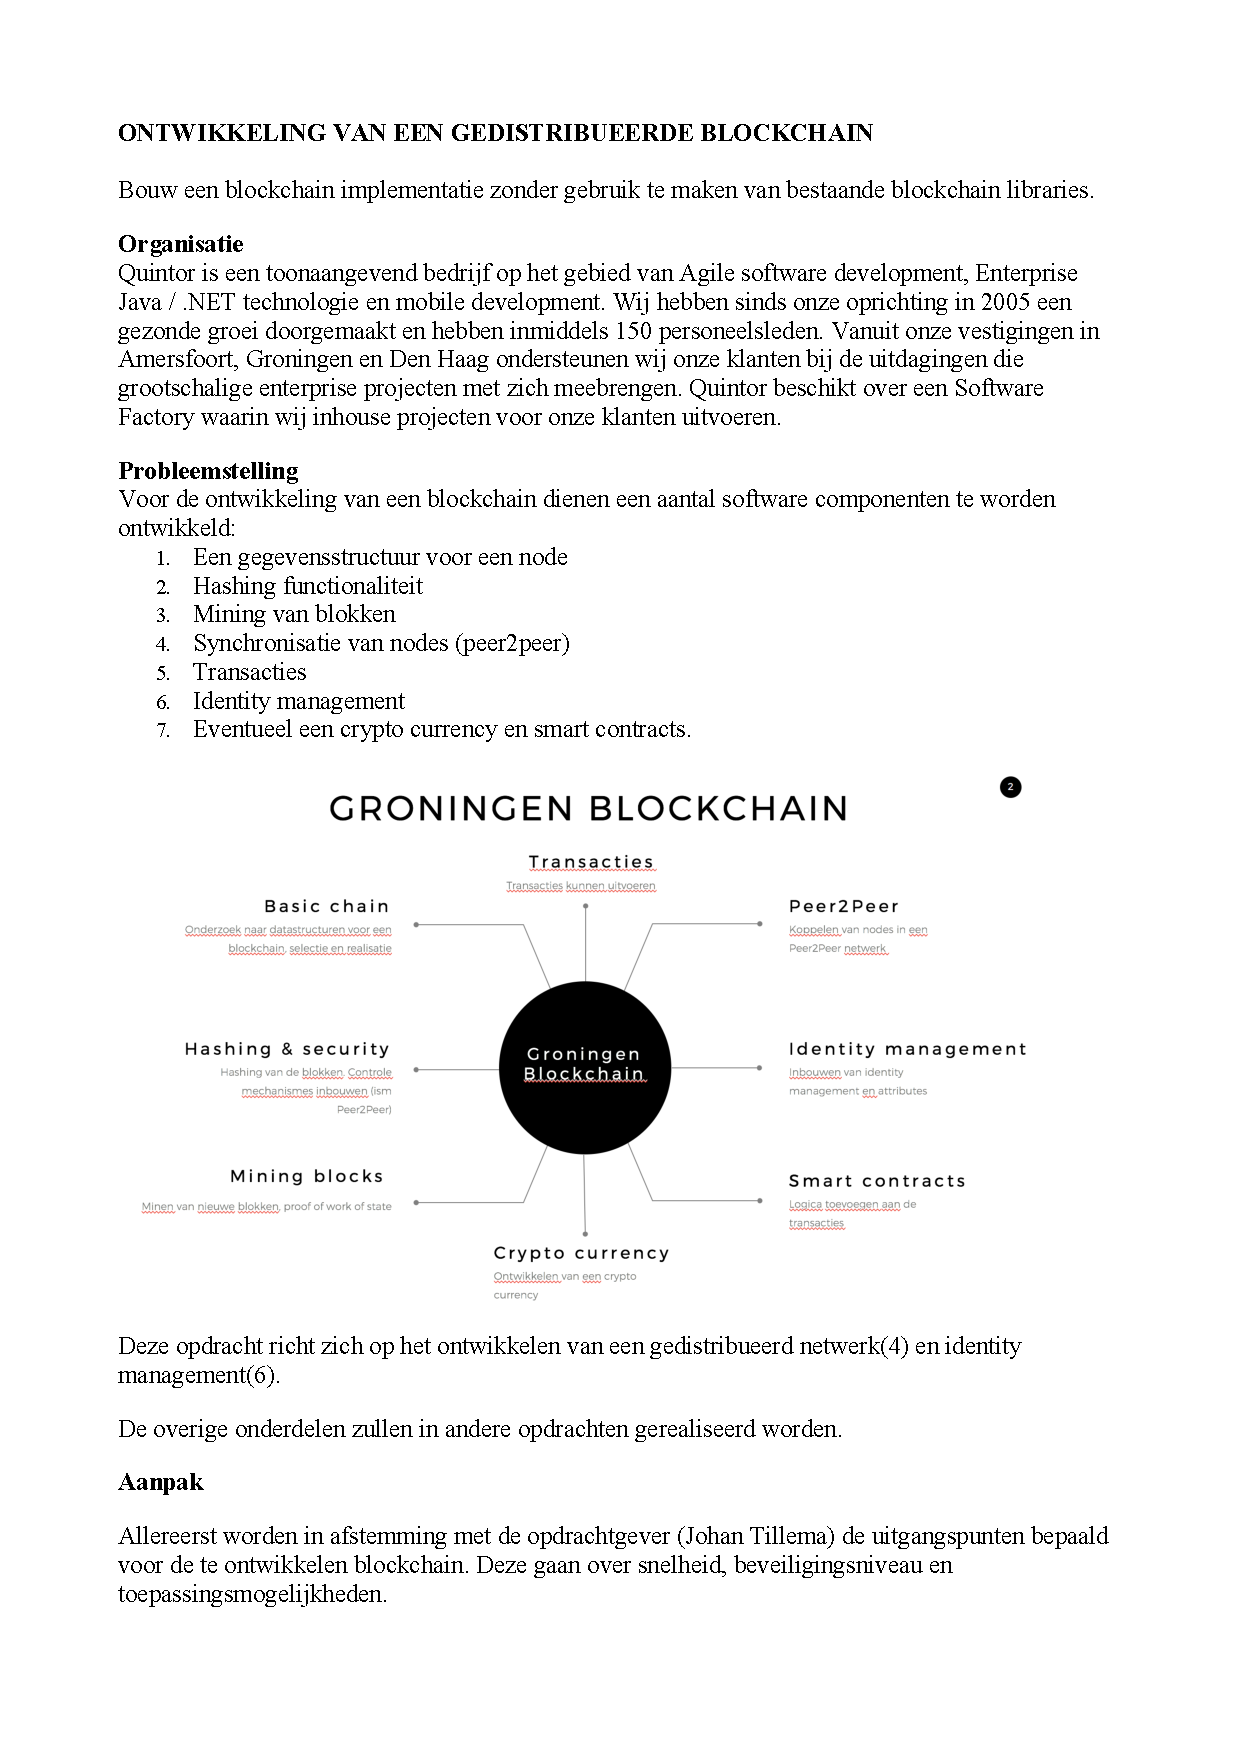
\includepdf[pages=-, frame=true, scale=0.7]{bijlages/quintor_opdracht.pdf}

  \section{Afstudeerplan}\label{appendix:afstudeerplan}
  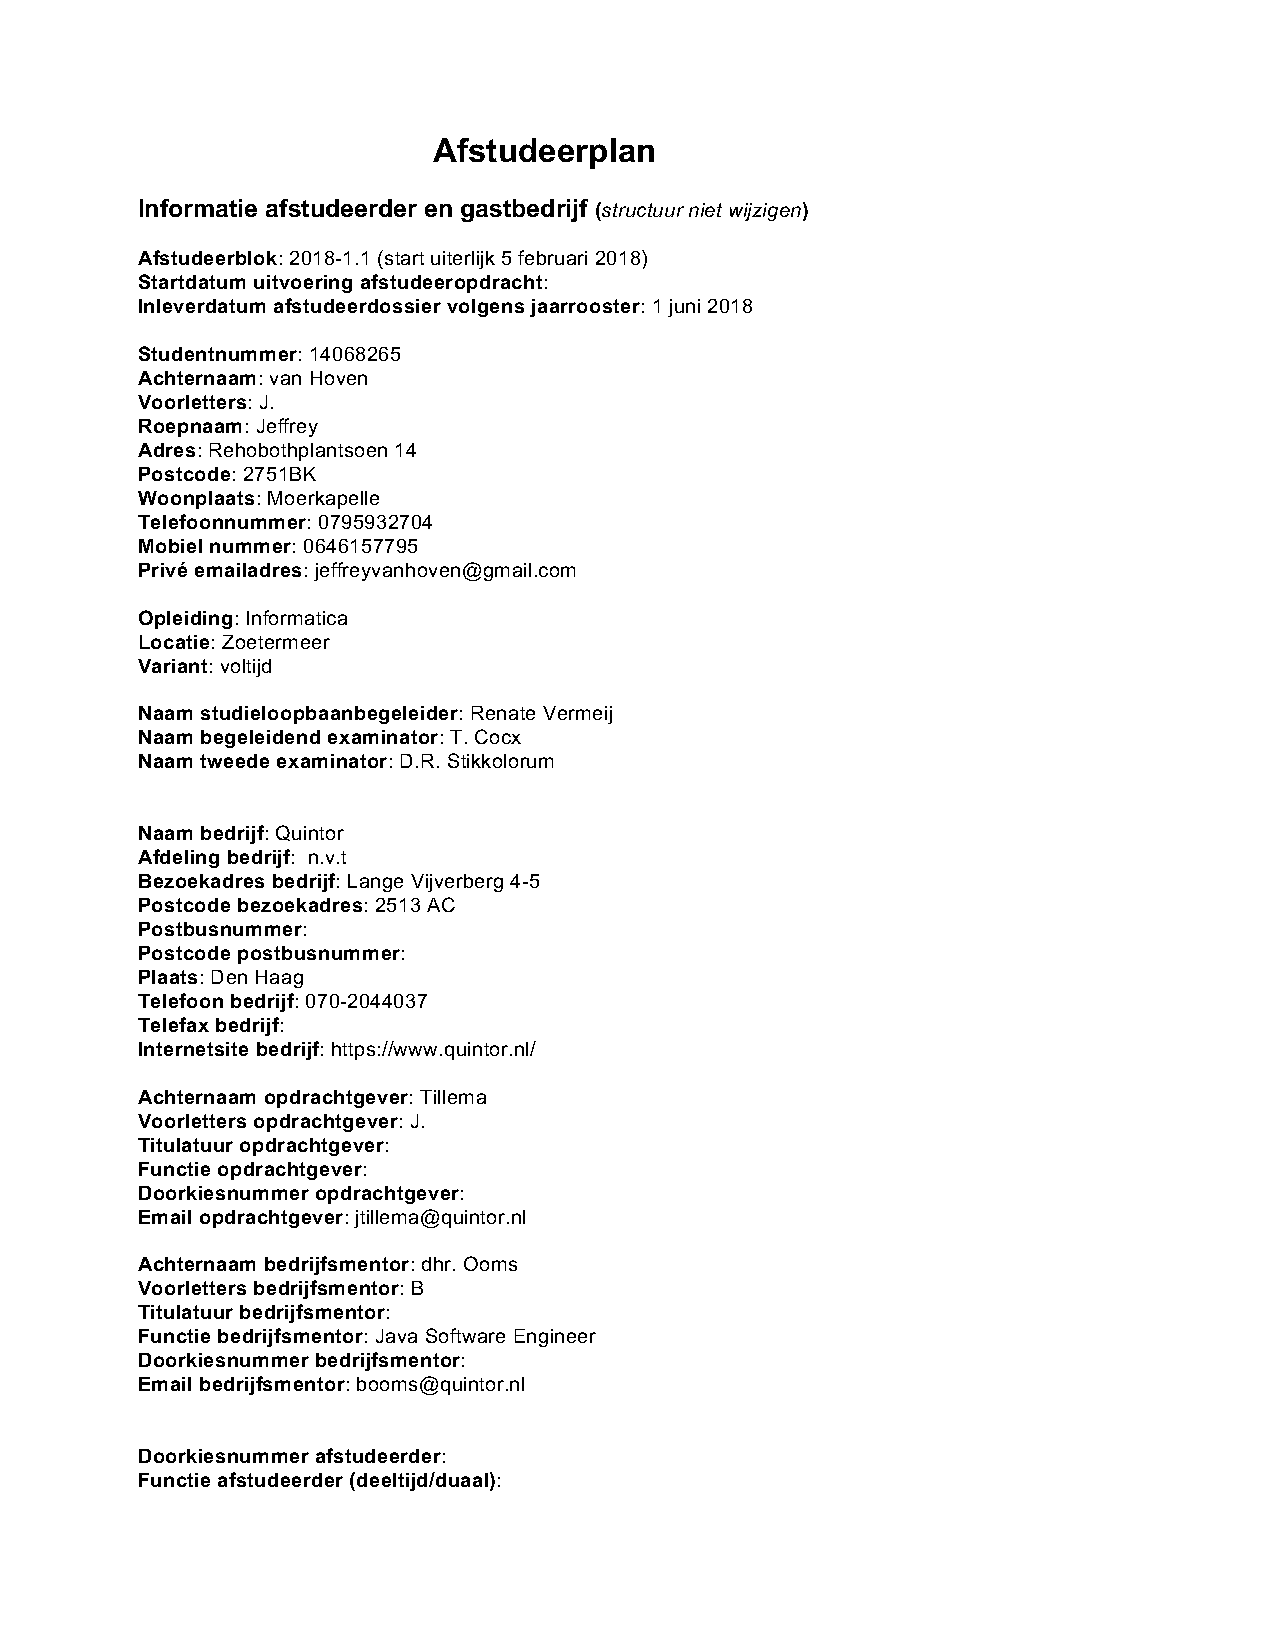
\includepdf[pages=-, frame=true, scale=0.7]{bijlages/afstudeerplan.pdf}

  \section{Plan van Aanpak}
  
\includepdf[pages=-, frame=true, scale=0.7]{bijlages/PvA/Aanpak.pdf}

  \section{Implementatie selectie}
  % Table generated by Excel2LaTeX from sheet 'Sheet2'
\begin{table}[htbp]
  \centering
  \caption{Bekeken implementaties uit de initiële selectie met de onderzochte attributen.}
  \begin{adjustbox}{width=25cm, height=6cm, angle=270}
    \begin{tabular}{llllrlp{17.915em}rlrrr}
      \toprule
      \textcolor[rgb]{ .188,  .329,  .588}{\textbf{Blockchain}} & \textcolor[rgb]{ .188,  .329,  .588}{\textbf{ Identity Management}} & \textcolor[rgb]{ .188,  .329,  .588}{\textbf{Whitepaper}} & \textcolor[rgb]{ .188,  .329,  .588}{\textbf{Open-source}} & \multicolumn{1}{l}{\textcolor[rgb]{ .188,  .329,  .588}{\textbf{In circulation since}}} & \textcolor[rgb]{ .188,  .329,  .588}{\textbf{Available Dapps development platform}} & \textcolor[rgb]{ .188,  .329,  .588}{\textbf{Notes}} & \multicolumn{1}{l}{\textcolor[rgb]{ .188,  .329,  .588}{\textbf{Consensus}}} & \textcolor[rgb]{ .188,  .329,  .588}{\textbf{Website}} & \multicolumn{1}{l}{\textcolor[rgb]{ .188,  .329,  .588}{\textbf{Repository}}} & \multicolumn{1}{l}{\textcolor[rgb]{ .188,  .329,  .588}{\textbf{Gebruikte talen}}} & \multicolumn{1}{l}{\textcolor[rgb]{ .188,  .329,  .588}{\textbf{Whitepaper url}}} \\
      \midrule
      \rowcolor[rgb]{ .267,  .447,  .769} \textcolor[rgb]{ 1,  1,  1}{\textbf{BitCoin}} & \cellcolor[rgb]{ 1,  .78,  .808}\textcolor[rgb]{ .612,  0,  .024}{No} & \cellcolor[rgb]{ .776,  .937,  .808}\textcolor[rgb]{ 0,  .38,  0}{Yes} & \cellcolor[rgb]{ .776,  .937,  .808}\textcolor[rgb]{ 0,  .38,  0}{Yes} & \cellcolor[rgb]{ .851,  .882,  .949}\textcolor[rgb]{ .188,  .329,  .588}{4/27/11} & \cellcolor[rgb]{ 1,  .78,  .808}\textcolor[rgb]{ .612,  0,  .024}{No} & \multicolumn{1}{r}{\cellcolor[rgb]{ .851,  .882,  .949}\textcolor[rgb]{ .188,  .329,  .588}{}} & \multicolumn{1}{l}{\cellcolor[rgb]{ .851,  .882,  .949}\textcolor[rgb]{ .188,  .329,  .588}{Proof of Work}} & \cellcolor[rgb]{ .851,  .882,  .949}\textcolor[rgb]{ .188,  .329,  .588}{https://bitcoin.org/nl/} & \multicolumn{1}{l}{\cellcolor[rgb]{ .851,  .882,  .949}\textcolor[rgb]{ .188,  .329,  .588}{https://github.com/bitcoin/}} & \multicolumn{1}{l}{\cellcolor[rgb]{ .851,  .882,  .949}\textcolor[rgb]{ .188,  .329,  .588}{C++}} & \multicolumn{1}{l}{\cellcolor[rgb]{ .851,  .882,  .949}\textcolor[rgb]{ .188,  .329,  .588}{https://bitcoin.org/bitcoin.pdf}} \\
      \rowcolor[rgb]{ .267,  .447,  .769} \textcolor[rgb]{ 1,  1,  1}{\textbf{Ethereum}} & \cellcolor[rgb]{ .776,  .937,  .808}\textcolor[rgb]{ 0,  .38,  0}{Yes} & \cellcolor[rgb]{ .776,  .937,  .808}\textcolor[rgb]{ 0,  .38,  0}{Yes} & \cellcolor[rgb]{ .776,  .937,  .808}\textcolor[rgb]{ 0,  .38,  0}{Yes} & \cellcolor[rgb]{ 1,  1,  1}\textcolor[rgb]{ .188,  .329,  .588}{7/30/15} & \cellcolor[rgb]{ .776,  .937,  .808}\textcolor[rgb]{ 0,  .38,  0}{Yes} & \multicolumn{1}{r}{\cellcolor[rgb]{ 1,  1,  1}\textcolor[rgb]{ .188,  .329,  .588}{}} & \multicolumn{1}{l}{\cellcolor[rgb]{ 1,  1,  1}\textcolor[rgb]{ .188,  .329,  .588}{Proof of Work}} & \cellcolor[rgb]{ 1,  1,  1}\textcolor[rgb]{ .188,  .329,  .588}{https://www.ethereum.org/} & \multicolumn{1}{l}{\cellcolor[rgb]{ 1,  1,  1}\textcolor[rgb]{ .188,  .329,  .588}{https://github.com/ethereum}} & \multicolumn{1}{l}{\cellcolor[rgb]{ 1,  1,  1}\textcolor[rgb]{ .188,  .329,  .588}{Go, C++}} & \multicolumn{1}{l}{\cellcolor[rgb]{ 1,  1,  1}\textcolor[rgb]{ .188,  .329,  .588}{https://github.com/ethereum/wiki/wiki/White-Paper}} \\
      \rowcolor[rgb]{ .267,  .447,  .769} \textcolor[rgb]{ 1,  1,  1}{\textbf{Tether}} & \cellcolor[rgb]{ 1,  .78,  .808}\textcolor[rgb]{ .612,  0,  .024}{No} & \cellcolor[rgb]{ .776,  .937,  .808}\textcolor[rgb]{ 0,  .38,  0}{Yes} & \cellcolor[rgb]{ 1,  .78,  .808}\textcolor[rgb]{ .612,  0,  .024}{No} & \cellcolor[rgb]{ .851,  .882,  .949}\textcolor[rgb]{ .188,  .329,  .588}{2015} & \cellcolor[rgb]{ .776,  .937,  .808}\textcolor[rgb]{ 0,  .38,  0}{Yes} & \cellcolor[rgb]{ .851,  .882,  .949}\textcolor[rgb]{ .188,  .329,  .588}{Fork from Bitcoin.} & \multicolumn{1}{l}{\cellcolor[rgb]{ .851,  .882,  .949}\textcolor[rgb]{ .188,  .329,  .588}{Proof of Reserves}} & \cellcolor[rgb]{ .851,  .882,  .949}\textcolor[rgb]{ .02,  .388,  .757}{https://www.tether.to/} & \multicolumn{1}{l}{\cellcolor[rgb]{ .851,  .882,  .949}\textcolor[rgb]{ .188,  .329,  .588}{https://bitbucket.org/tetherto/}} & \cellcolor[rgb]{ .851,  .882,  .949}\textcolor[rgb]{ .188,  .329,  .588}{} & \multicolumn{1}{l}{\cellcolor[rgb]{ .851,  .882,  .949}\textcolor[rgb]{ .188,  .329,  .588}{https://tether.to/wp-content/uploads/2016/06/TetherWhitePaper.pdf}} \\
      \rowcolor[rgb]{ .267,  .447,  .769} \textcolor[rgb]{ 1,  1,  1}{\textbf{Ripple}} & \cellcolor[rgb]{ 1,  .922,  .612}\textcolor[rgb]{ .612,  .341,  0}{Not sure} & \cellcolor[rgb]{ .776,  .937,  .808}\textcolor[rgb]{ 0,  .38,  0}{Yes} & \cellcolor[rgb]{ .776,  .937,  .808}\textcolor[rgb]{ 0,  .38,  0}{Yes} & \cellcolor[rgb]{ .851,  .882,  .949}\textcolor[rgb]{ .188,  .329,  .588}{2012} & \cellcolor[rgb]{ 1,  .78,  .808}\textcolor[rgb]{ .612,  0,  .024}{No} & \cellcolor[rgb]{ .851,  .882,  .949}\textcolor[rgb]{ .188,  .329,  .588}{Not really a Blockchain} & \multicolumn{1}{l}{\cellcolor[rgb]{ .851,  .882,  .949}\textcolor[rgb]{ .188,  .329,  .588}{Ripple Consensus Algorithm}} & \cellcolor[rgb]{ .851,  .882,  .949}\textcolor[rgb]{ .188,  .329,  .588}{https://ripple.com/} & \multicolumn{1}{l}{\cellcolor[rgb]{ .851,  .882,  .949}\textcolor[rgb]{ .188,  .329,  .588}{https://github.com/ripple}} & \multicolumn{1}{l}{\cellcolor[rgb]{ .851,  .882,  .949}\textcolor[rgb]{ .188,  .329,  .588}{C++}} & \multicolumn{1}{l}{\cellcolor[rgb]{ .851,  .882,  .949}\textcolor[rgb]{ .188,  .329,  .588}{https://ripple.com/files/ripple\_consensus\_whitepaper.pdf}} \\
      \rowcolor[rgb]{ .267,  .447,  .769} \textcolor[rgb]{ 1,  1,  1}{\textbf{EOS}} & \cellcolor[rgb]{ .776,  .937,  .808}\textcolor[rgb]{ 0,  .38,  0}{Yes} & \cellcolor[rgb]{ 1,  .922,  .612}\textcolor[rgb]{ .612,  .341,  0}{Sort of} & \cellcolor[rgb]{ .776,  .937,  .808}\textcolor[rgb]{ 0,  .38,  0}{Yes} & \cellcolor[rgb]{ 1,  1,  1}\textcolor[rgb]{ .188,  .329,  .588}{1/31/18} & \cellcolor[rgb]{ .776,  .937,  .808}\textcolor[rgb]{ 0,  .38,  0}{Yes} & \multicolumn{1}{r}{\cellcolor[rgb]{ 1,  1,  1}\textcolor[rgb]{ .188,  .329,  .588}{}} & \multicolumn{1}{l}{\cellcolor[rgb]{ 1,  1,  1}\textcolor[rgb]{ .188,  .329,  .588}{Delegated Proof of Stake}} & \cellcolor[rgb]{ 1,  1,  1}\textcolor[rgb]{ .188,  .329,  .588}{https://eos.io/} & \multicolumn{1}{l}{\cellcolor[rgb]{ 1,  1,  1}\textcolor[rgb]{ .188,  .329,  .588}{https://github.com/EOSIO}} & \multicolumn{1}{l}{\cellcolor[rgb]{ 1,  1,  1}\textcolor[rgb]{ .188,  .329,  .588}{C++}} & \cellcolor[rgb]{ 1,  1,  1}\textcolor[rgb]{ .188,  .329,  .588}{} \\
      \rowcolor[rgb]{ .267,  .447,  .769} \textcolor[rgb]{ 1,  1,  1}{\textbf{Cardano}} & \cellcolor[rgb]{ 1,  .922,  .612}\textcolor[rgb]{ .612,  .341,  0}{Not sure} & \cellcolor[rgb]{ .776,  .937,  .808}\textcolor[rgb]{ 0,  .38,  0}{Yes} & \cellcolor[rgb]{ 1,  .922,  .612}\textcolor[rgb]{ .612,  .341,  0}{Sort of} & \cellcolor[rgb]{ .851,  .882,  .949}\textcolor[rgb]{ .188,  .329,  .588}{11/29/17} & \cellcolor[rgb]{ .776,  .937,  .808}\textcolor[rgb]{ 0,  .38,  0}{Yes} & \cellcolor[rgb]{ .851,  .882,  .949}\textcolor[rgb]{ .188,  .329,  .588}{Only the "Settlement Layer" is open-source available} & \multicolumn{1}{l}{\cellcolor[rgb]{ .851,  .882,  .949}\textcolor[rgb]{ .188,  .329,  .588}{Proof of Stake}} & \cellcolor[rgb]{ .851,  .882,  .949}\textcolor[rgb]{ .188,  .329,  .588}{} & \multicolumn{1}{l}{\cellcolor[rgb]{ .851,  .882,  .949}\textcolor[rgb]{ .188,  .329,  .588}{https://github.com/input-output-hk/cardano-sl }} & \multicolumn{1}{l}{\cellcolor[rgb]{ .851,  .882,  .949}\textcolor[rgb]{ .188,  .329,  .588}{Haskell}} & \cellcolor[rgb]{ .851,  .882,  .949}\textcolor[rgb]{ .188,  .329,  .588}{} \\
      \rowcolor[rgb]{ .267,  .447,  .769} \textcolor[rgb]{ 1,  1,  1}{\textbf{NEO}} & \cellcolor[rgb]{ .776,  .937,  .808}\textcolor[rgb]{ 0,  .38,  0}{Yes} & \cellcolor[rgb]{ 1,  .78,  .808}\textcolor[rgb]{ .612,  0,  .024}{No} & \cellcolor[rgb]{ .776,  .937,  .808}\textcolor[rgb]{ 0,  .38,  0}{Yes} & \cellcolor[rgb]{ 1,  1,  1}\textcolor[rgb]{ .188,  .329,  .588}{2014} & \cellcolor[rgb]{ .776,  .937,  .808}\textcolor[rgb]{ 0,  .38,  0}{Yes} & \multicolumn{1}{r}{\cellcolor[rgb]{ 1,  1,  1}\textcolor[rgb]{ .188,  .329,  .588}{}} & \multicolumn{1}{l}{\cellcolor[rgb]{ 1,  1,  1}\textcolor[rgb]{ .188,  .329,  .588}{Delegated Byzantine Fault Tolerance}} & \cellcolor[rgb]{ 1,  1,  1}\textcolor[rgb]{ .188,  .329,  .588}{https://neo.org/} & \multicolumn{1}{l}{\cellcolor[rgb]{ 1,  1,  1}\textcolor[rgb]{ .188,  .329,  .588}{https://github.com/neo-project}} & \cellcolor[rgb]{ 1,  1,  1}\textcolor[rgb]{ .188,  .329,  .588}{} & \cellcolor[rgb]{ 1,  1,  1}\textcolor[rgb]{ .188,  .329,  .588}{} \\
      \rowcolor[rgb]{ .267,  .447,  .769} \textcolor[rgb]{ 1,  1,  1}{\textbf{Qtum}} & \cellcolor[rgb]{ .776,  .937,  .808}\textcolor[rgb]{ 0,  .38,  0}{Yes} & \cellcolor[rgb]{ .776,  .937,  .808}\textcolor[rgb]{ 0,  .38,  0}{Yes} & \cellcolor[rgb]{ 1,  .922,  .612}\textcolor[rgb]{ .612,  .341,  0}{Sort of} & \cellcolor[rgb]{ 1,  1,  1}11/13/17 & \cellcolor[rgb]{ .776,  .937,  .808}\textcolor[rgb]{ 0,  .38,  0}{Yes} & \cellcolor[rgb]{ .851,  .882,  .949}\textcolor[rgb]{ .188,  .329,  .588}{Adopts the UTXO model from Bitcoin while utilizing the Ethereum network. Implements PoS 3.0 as coined by the original Proof of Stake coin Blackcoin. Only the wallet is open-source.} & \multicolumn{1}{l}{\cellcolor[rgb]{ .851,  .882,  .949}\textcolor[rgb]{ .188,  .329,  .588}{Proof of Stake}} & \cellcolor[rgb]{ 1,  1,  1}https://qtum.org/en/ & \multicolumn{1}{l}{\cellcolor[rgb]{ 1,  1,  1}https://github.com/qtumproject} & \multicolumn{1}{l}{\cellcolor[rgb]{ .851,  .882,  .949}\textcolor[rgb]{ .188,  .329,  .588}{Wallet in C++}} & \multicolumn{1}{l}{\cellcolor[rgb]{ 1,  1,  1}https://qtum.org/uploads/files/a2772efe4dc8ed1100319c6480195fb1.pdf} \\
      \rowcolor[rgb]{ .267,  .447,  .769} \textcolor[rgb]{ 1,  1,  1}{\textbf{TRON}} & \cellcolor[rgb]{ 1,  .78,  .808}\textcolor[rgb]{ .612,  0,  .024}{No} & \cellcolor[rgb]{ .776,  .937,  .808}\textcolor[rgb]{ 0,  .38,  0}{Yes} & \cellcolor[rgb]{ 1,  .922,  .612}\textcolor[rgb]{ .612,  .341,  0}{Sort of} & \cellcolor[rgb]{ .851,  .882,  .949}\textcolor[rgb]{ .188,  .329,  .588}{2017} & \cellcolor[rgb]{ 1,  .78,  .808}\textcolor[rgb]{ .612,  0,  .024}{No} & \cellcolor[rgb]{ 1,  1,  1}\textcolor[rgb]{ .188,  .329,  .588}{Badly translated whitepaper and website.} & \multicolumn{1}{l}{\cellcolor[rgb]{ .851,  .882,  .949}\textcolor[rgb]{ .188,  .329,  .588}{Proof of Stake}} & \cellcolor[rgb]{ .851,  .882,  .949}\textcolor[rgb]{ .188,  .329,  .588}{https://tron.network/en.html} & \multicolumn{1}{l}{\cellcolor[rgb]{ .851,  .882,  .949}\textcolor[rgb]{ .188,  .329,  .588}{https://github.com/tronprotocol}} & \multicolumn{1}{l}{\cellcolor[rgb]{ .851,  .882,  .949}\textcolor[rgb]{ .188,  .329,  .588}{Java}} & \multicolumn{1}{l}{\cellcolor[rgb]{ .851,  .882,  .949}\textcolor[rgb]{ .188,  .329,  .588}{https://o836fhe91.qnssl.com/tron/whitebook/TronWhitepaper\_en.pdf}} \\
      \rowcolor[rgb]{ .267,  .447,  .769} \textcolor[rgb]{ 1,  1,  1}{\textbf{Status}} & \cellcolor[rgb]{ .776,  .937,  .808}\textcolor[rgb]{ 0,  .38,  0}{Yes} & \cellcolor[rgb]{ 1,  .78,  .808}\textcolor[rgb]{ .612,  0,  .024}{No} & \cellcolor[rgb]{ .776,  .937,  .808}\textcolor[rgb]{ 0,  .38,  0}{Yes} & \multicolumn{1}{l}{\cellcolor[rgb]{ 1,  1,  1}-} & \cellcolor[rgb]{ .776,  .937,  .808}\textcolor[rgb]{ 0,  .38,  0}{Yes} & \cellcolor[rgb]{ .851,  .882,  .949}\textcolor[rgb]{ .188,  .329,  .588}{Identity Management in form of usernames. Mobile client voor Ethereum, een Dapp die het mogelijk maakt om te interfacen met andere Dapps?} & \multicolumn{1}{l}{\cellcolor[rgb]{ .851,  .882,  .949}\textcolor[rgb]{ .188,  .329,  .588}{Proof of Work}} & \cellcolor[rgb]{ 1,  1,  1}https://status.im/ & \multicolumn{1}{l}{\cellcolor[rgb]{ 1,  1,  1}https://github.com/status-im} & \multicolumn{1}{l}{\cellcolor[rgb]{ .851,  .882,  .949}\textcolor[rgb]{ .188,  .329,  .588}{Go}} & \cellcolor[rgb]{ 1,  1,  1} \\
      \rowcolor[rgb]{ .267,  .447,  .769} \textcolor[rgb]{ 1,  1,  1}{\textbf{Stellar}} & \cellcolor[rgb]{ 1,  .922,  .612}\textcolor[rgb]{ .612,  .341,  0}{Not sure} & \cellcolor[rgb]{ 1,  .922,  .612}\textcolor[rgb]{ .612,  .341,  0}{Sort of} & \cellcolor[rgb]{ .776,  .937,  .808}\textcolor[rgb]{ 0,  .38,  0}{Yes} & \cellcolor[rgb]{ .851,  .882,  .949}\textcolor[rgb]{ .188,  .329,  .588}{2014} & \cellcolor[rgb]{ .776,  .937,  .808}\textcolor[rgb]{ 0,  .38,  0}{Yes} & \cellcolor[rgb]{ 1,  1,  1}\textcolor[rgb]{ .188,  .329,  .588}{Whitepaper only describes the consensus protocol, initially based on te Ripple protocol} & \multicolumn{1}{l}{\cellcolor[rgb]{ .851,  .882,  .949}\textcolor[rgb]{ .188,  .329,  .588}{Stellar Consensus Protocol}} & \cellcolor[rgb]{ .851,  .882,  .949}\textcolor[rgb]{ .188,  .329,  .588}{https://www.stellar.org} & \multicolumn{1}{l}{\cellcolor[rgb]{ .851,  .882,  .949}\textcolor[rgb]{ .188,  .329,  .588}{https://github.com/stellar}} & \multicolumn{1}{l}{\cellcolor[rgb]{ .851,  .882,  .949}\textcolor[rgb]{ .188,  .329,  .588}{C}} & \cellcolor[rgb]{ .851,  .882,  .949}\textcolor[rgb]{ .188,  .329,  .588}{} \\
      \rowcolor[rgb]{ .267,  .447,  .769} \textcolor[rgb]{ 1,  1,  1}{\textbf{Huobi Token}} & \cellcolor[rgb]{ 1,  .78,  .808}\textcolor[rgb]{ .612,  0,  .024}{No} & \cellcolor[rgb]{ 1,  .78,  .808}\textcolor[rgb]{ .612,  0,  .024}{No} & \cellcolor[rgb]{ 1,  .78,  .808}\textcolor[rgb]{ .612,  0,  .024}{No} & \cellcolor[rgb]{ 1,  1,  1} & \cellcolor[rgb]{ 1,  .78,  .808}\textcolor[rgb]{ .612,  0,  .024}{No} & \cellcolor[rgb]{ .851,  .882,  .949}\textcolor[rgb]{ .188,  .329,  .588}{Loyalty Blockchain, users cant buy but are awarded these tokens.} & \multicolumn{1}{l}{\cellcolor[rgb]{ .851,  .882,  .949}\textcolor[rgb]{ .188,  .329,  .588}{?}} & \cellcolor[rgb]{ 1,  1,  1}https://www.huobi.pro & \cellcolor[rgb]{ 1,  1,  1} & \cellcolor[rgb]{ 1,  1,  1} & \cellcolor[rgb]{ 1,  1,  1} \\
      \rowcolor[rgb]{ .267,  .447,  .769} \textcolor[rgb]{ 1,  1,  1}{\textbf{ATMCoin}} & \cellcolor[rgb]{ 1,  .922,  .612}\textcolor[rgb]{ .612,  .341,  0}{Not sure} & \cellcolor[rgb]{ 1,  .78,  .808}\textcolor[rgb]{ .612,  0,  .024}{No} & \cellcolor[rgb]{ 1,  .78,  .808}\textcolor[rgb]{ .612,  0,  .024}{No} & \multicolumn{1}{l}{\cellcolor[rgb]{ 1,  1,  1}-} & \cellcolor[rgb]{ 1,  .78,  .808}\textcolor[rgb]{ .612,  0,  .024}{No} & \cellcolor[rgb]{ 1,  1,  1}\textcolor[rgb]{ .188,  .329,  .588}{Doesnt look like anythings available for this crypto.} & \cellcolor[rgb]{ 1,  1,  1} & \cellcolor[rgb]{ 1,  1,  1}https://atmcoin.com/website/inicio & \cellcolor[rgb]{ 1,  1,  1} & \cellcolor[rgb]{ 1,  1,  1} & \multicolumn{1}{l}{\cellcolor[rgb]{ 1,  1,  1}https://atmcoin.com/contenidos/documentos/atmcoin\_whitepaper\_en-us.pdf} \\
      \rowcolor[rgb]{ .267,  .447,  .769} \textcolor[rgb]{ 1,  1,  1}{\textbf{Dash}} & \cellcolor[rgb]{ 1,  .78,  .808}\textcolor[rgb]{ .612,  0,  .024}{No} & \cellcolor[rgb]{ 1,  .922,  .612}\textcolor[rgb]{ .612,  .341,  0}{Sort of} & \cellcolor[rgb]{ .776,  .937,  .808}\textcolor[rgb]{ 0,  .38,  0}{Yes} & \cellcolor[rgb]{ .851,  .882,  .949}\textcolor[rgb]{ .188,  .329,  .588}{1/18/14} & \cellcolor[rgb]{ 1,  .922,  .612}\textcolor[rgb]{ .612,  .341,  0}{Not sure} & \cellcolor[rgb]{ .851,  .882,  .949}\textcolor[rgb]{ .188,  .329,  .588}{Initially named Xcoin (XCO), renamed to Darkcoin and then rebranded as Dash. Fork from LiteCoin. First self funded blockchain. Transaction fees go to a treasury, which funds development} & \multicolumn{1}{l}{\cellcolor[rgb]{ .851,  .882,  .949}\textcolor[rgb]{ .188,  .329,  .588}{Proof of Service}} & \cellcolor[rgb]{ .851,  .882,  .949}\textcolor[rgb]{ .188,  .329,  .588}{https://www.dash.org/} & \multicolumn{1}{l}{\cellcolor[rgb]{ .851,  .882,  .949}\textcolor[rgb]{ .188,  .329,  .588}{https://github.com/dashpay}} & \multicolumn{1}{l}{\cellcolor[rgb]{ .851,  .882,  .949}\textcolor[rgb]{ .188,  .329,  .588}{C++}} & \multicolumn{1}{l}{\cellcolor[rgb]{ .851,  .882,  .949}\textcolor[rgb]{ .188,  .329,  .588}{https://github.com/dashpay/dash/wiki/Whitepaper}} \\
      \rowcolor[rgb]{ .267,  .447,  .769} \textcolor[rgb]{ 1,  1,  1}{\textbf{VeChain}} & \cellcolor[rgb]{ 1,  .78,  .808}\textcolor[rgb]{ .612,  0,  .024}{No} & \cellcolor[rgb]{ 1,  .78,  .808}\textcolor[rgb]{ .612,  0,  .024}{No} & \cellcolor[rgb]{ 1,  .78,  .808}\textcolor[rgb]{ .612,  0,  .024}{No} & \cellcolor[rgb]{ 1,  1,  1}\textcolor[rgb]{ .188,  .329,  .588}{2015} & \cellcolor[rgb]{ 1,  .78,  .808}\textcolor[rgb]{ .612,  0,  .024}{No} & \cellcolor[rgb]{ 1,  1,  1}\textcolor[rgb]{ .188,  .329,  .588}{Chinese, private Blockchain for retail usage in combination with IoT.} & \cellcolor[rgb]{ 1,  1,  1}\textcolor[rgb]{ .188,  .329,  .588}{} & \cellcolor[rgb]{ 1,  1,  1}\textcolor[rgb]{ .188,  .329,  .588}{https://www.vechain.com/\#/} & \cellcolor[rgb]{ 1,  1,  1}\textcolor[rgb]{ .188,  .329,  .588}{} & \cellcolor[rgb]{ 1,  1,  1}\textcolor[rgb]{ .188,  .329,  .588}{} & \cellcolor[rgb]{ 1,  1,  1}\textcolor[rgb]{ .188,  .329,  .588}{} \\
      \rowcolor[rgb]{ .267,  .447,  .769} \textcolor[rgb]{ 1,  1,  1}{\textbf{Lisk}} & \cellcolor[rgb]{ .776,  .937,  .808}\textcolor[rgb]{ 0,  .38,  0}{Yes} & \cellcolor[rgb]{ 1,  .78,  .808}\textcolor[rgb]{ .612,  0,  .024}{No} & \cellcolor[rgb]{ .776,  .937,  .808}\textcolor[rgb]{ 0,  .38,  0}{Yes} & \cellcolor[rgb]{ 1,  1,  1}9/22/17 & \cellcolor[rgb]{ .776,  .937,  .808}\textcolor[rgb]{ 0,  .38,  0}{Yes} & \cellcolor[rgb]{ .851,  .882,  .949}\textcolor[rgb]{ .188,  .329,  .588}{Technical documentation available at https://lisk.io/documentation, albeit not in-depth.} & \multicolumn{1}{l}{\cellcolor[rgb]{ .851,  .882,  .949}\textcolor[rgb]{ .188,  .329,  .588}{Delegated Proof of Stake}} & \cellcolor[rgb]{ 1,  1,  1}https://lisk.io/ & \multicolumn{1}{l}{\cellcolor[rgb]{ 1,  1,  1}https://github.com/LiskHQ} & \multicolumn{1}{l}{\cellcolor[rgb]{ .851,  .882,  .949}\textcolor[rgb]{ .188,  .329,  .588}{JavaScript}} & \multicolumn{1}{l}{\cellcolor[rgb]{ 1,  1,  1}https://lisk.io/documentation/} \\
      \rowcolor[rgb]{ .267,  .447,  .769} \textcolor[rgb]{ 1,  1,  1}{\textbf{Monero}} & \cellcolor[rgb]{ .776,  .937,  .808}\textcolor[rgb]{ 0,  .38,  0}{Yes} & \cellcolor[rgb]{ .776,  .937,  .808}\textcolor[rgb]{ 0,  .38,  0}{Yes} & \cellcolor[rgb]{ .776,  .937,  .808}\textcolor[rgb]{ 0,  .38,  0}{Yes} & \cellcolor[rgb]{ .851,  .882,  .949}\textcolor[rgb]{ .188,  .329,  .588}{4/18/14} & \cellcolor[rgb]{ 1,  .78,  .808}\textcolor[rgb]{ .612,  0,  .024}{No} & \cellcolor[rgb]{ 1,  1,  1}\textcolor[rgb]{ .188,  .329,  .588}{Claims to be one and only fully anonimized Blockchain implementation} & \multicolumn{1}{l}{\cellcolor[rgb]{ .851,  .882,  .949}\textcolor[rgb]{ .188,  .329,  .588}{Proof of Work}} & \cellcolor[rgb]{ .851,  .882,  .949}\textcolor[rgb]{ .188,  .329,  .588}{https://getmonero.org/} & \multicolumn{1}{l}{\cellcolor[rgb]{ .851,  .882,  .949}\textcolor[rgb]{ .188,  .329,  .588}{https://github.com/monero-project}} & \multicolumn{1}{l}{\cellcolor[rgb]{ .851,  .882,  .949}\textcolor[rgb]{ .188,  .329,  .588}{C++}} & \multicolumn{1}{l}{\cellcolor[rgb]{ .851,  .882,  .949}\textcolor[rgb]{ .188,  .329,  .588}{https://downloads.getmonero.org/whitepaper\_annotated.pdf}} \\
      \rowcolor[rgb]{ .267,  .447,  .769} \textcolor[rgb]{ 1,  1,  1}{\textbf{Hshare}} & \cellcolor[rgb]{ .776,  .937,  .808}\textcolor[rgb]{ 0,  .38,  0}{Yes} & \cellcolor[rgb]{ .776,  .937,  .808}\textcolor[rgb]{ 0,  .38,  0}{Yes} & \cellcolor[rgb]{ .776,  .937,  .808}\textcolor[rgb]{ 0,  .38,  0}{Yes} & \cellcolor[rgb]{ 1,  1,  1} & \cellcolor[rgb]{ 1,  1,  1} & \cellcolor[rgb]{ .851,  .882,  .949}\textcolor[rgb]{ .188,  .329,  .588}{Uses black and white addresses} & \multicolumn{1}{l}{\cellcolor[rgb]{ .851,  .882,  .949}\textcolor[rgb]{ .188,  .329,  .588}{PoW + PoS}} & \cellcolor[rgb]{ 1,  1,  1}https://h.cash/ & \multicolumn{1}{l}{\cellcolor[rgb]{ 1,  1,  1}https://github.com/HcashOrg} & \multicolumn{1}{l}{\cellcolor[rgb]{ .851,  .882,  .949}\textcolor[rgb]{ .188,  .329,  .588}{C++}} & \cellcolor[rgb]{ 1,  1,  1} \\
      \rowcolor[rgb]{ .267,  .447,  .769} \textcolor[rgb]{ 1,  1,  1}{\textbf{ICON}} & \cellcolor[rgb]{ .776,  .937,  .808}\textcolor[rgb]{ 0,  .38,  0}{Yes} & \cellcolor[rgb]{ .776,  .937,  .808}\textcolor[rgb]{ 0,  .38,  0}{Yes} & \cellcolor[rgb]{ 1,  .78,  .808}\textcolor[rgb]{ .612,  0,  .024}{No} & \cellcolor[rgb]{ 1,  1,  1}\textcolor[rgb]{ .188,  .329,  .588}{} & \cellcolor[rgb]{ 1,  .922,  .612}\textcolor[rgb]{ .612,  .341,  0}{Not sure} & \multicolumn{1}{r}{\cellcolor[rgb]{ 1,  1,  1}\textcolor[rgb]{ .188,  .329,  .588}{}} & \multicolumn{1}{l}{\cellcolor[rgb]{ 1,  1,  1}\textcolor[rgb]{ .188,  .329,  .588}{Loop Fault Tolerance}} & \cellcolor[rgb]{ 1,  1,  1}\textcolor[rgb]{ .188,  .329,  .588}{https://icon.foundation/?lang=en} & \multicolumn{1}{l}{\cellcolor[rgb]{ 1,  1,  1}\textcolor[rgb]{ .188,  .329,  .588}{https://github.com/icon-foundation/}} & \cellcolor[rgb]{ 1,  1,  1}\textcolor[rgb]{ .188,  .329,  .588}{} & \multicolumn{1}{l}{\cellcolor[rgb]{ 1,  1,  1}\textcolor[rgb]{ .188,  .329,  .588}{https://icon.foundation/resources/whitepaper/ICON-Whitepaper-EN-Draft.pdf}} \\
      \rowcolor[rgb]{ .267,  .447,  .769} \textcolor[rgb]{ 1,  1,  1}{\textbf{Nano}} & \cellcolor[rgb]{ 1,  .78,  .808}\textcolor[rgb]{ .612,  0,  .024}{No} & \cellcolor[rgb]{ .776,  .937,  .808}\textcolor[rgb]{ 0,  .38,  0}{Yes} & \cellcolor[rgb]{ .776,  .937,  .808}\textcolor[rgb]{ 0,  .38,  0}{Yes} & \cellcolor[rgb]{ 1,  1,  1}\textcolor[rgb]{ .188,  .329,  .588}{} & \cellcolor[rgb]{ 1,  .78,  .808}\textcolor[rgb]{ .612,  0,  .024}{No} & \cellcolor[rgb]{ .851,  .882,  .949}\textcolor[rgb]{ .188,  .329,  .588}{Previously known as Raiblocks. Second blockchain that uses a tangle instead of a chain.} & \cellcolor[rgb]{ 1,  1,  1}\textcolor[rgb]{ .188,  .329,  .588}{} & \cellcolor[rgb]{ 1,  1,  1}\textcolor[rgb]{ .188,  .329,  .588}{https://nano.org/en} & \cellcolor[rgb]{ 1,  1,  1}\textcolor[rgb]{ .188,  .329,  .588}{} & \cellcolor[rgb]{ 1,  1,  1}\textcolor[rgb]{ .188,  .329,  .588}{} & \cellcolor[rgb]{ 1,  1,  1}\textcolor[rgb]{ .188,  .329,  .588}{} \\
      \cmidrule{2-6}\cmidrule{8-12}    
    \end{tabular}
  \end{adjustbox}
  \label{bijlage_selectie_implementatie}
\end{table}




  
  \section{Onderzoeksrapport}
  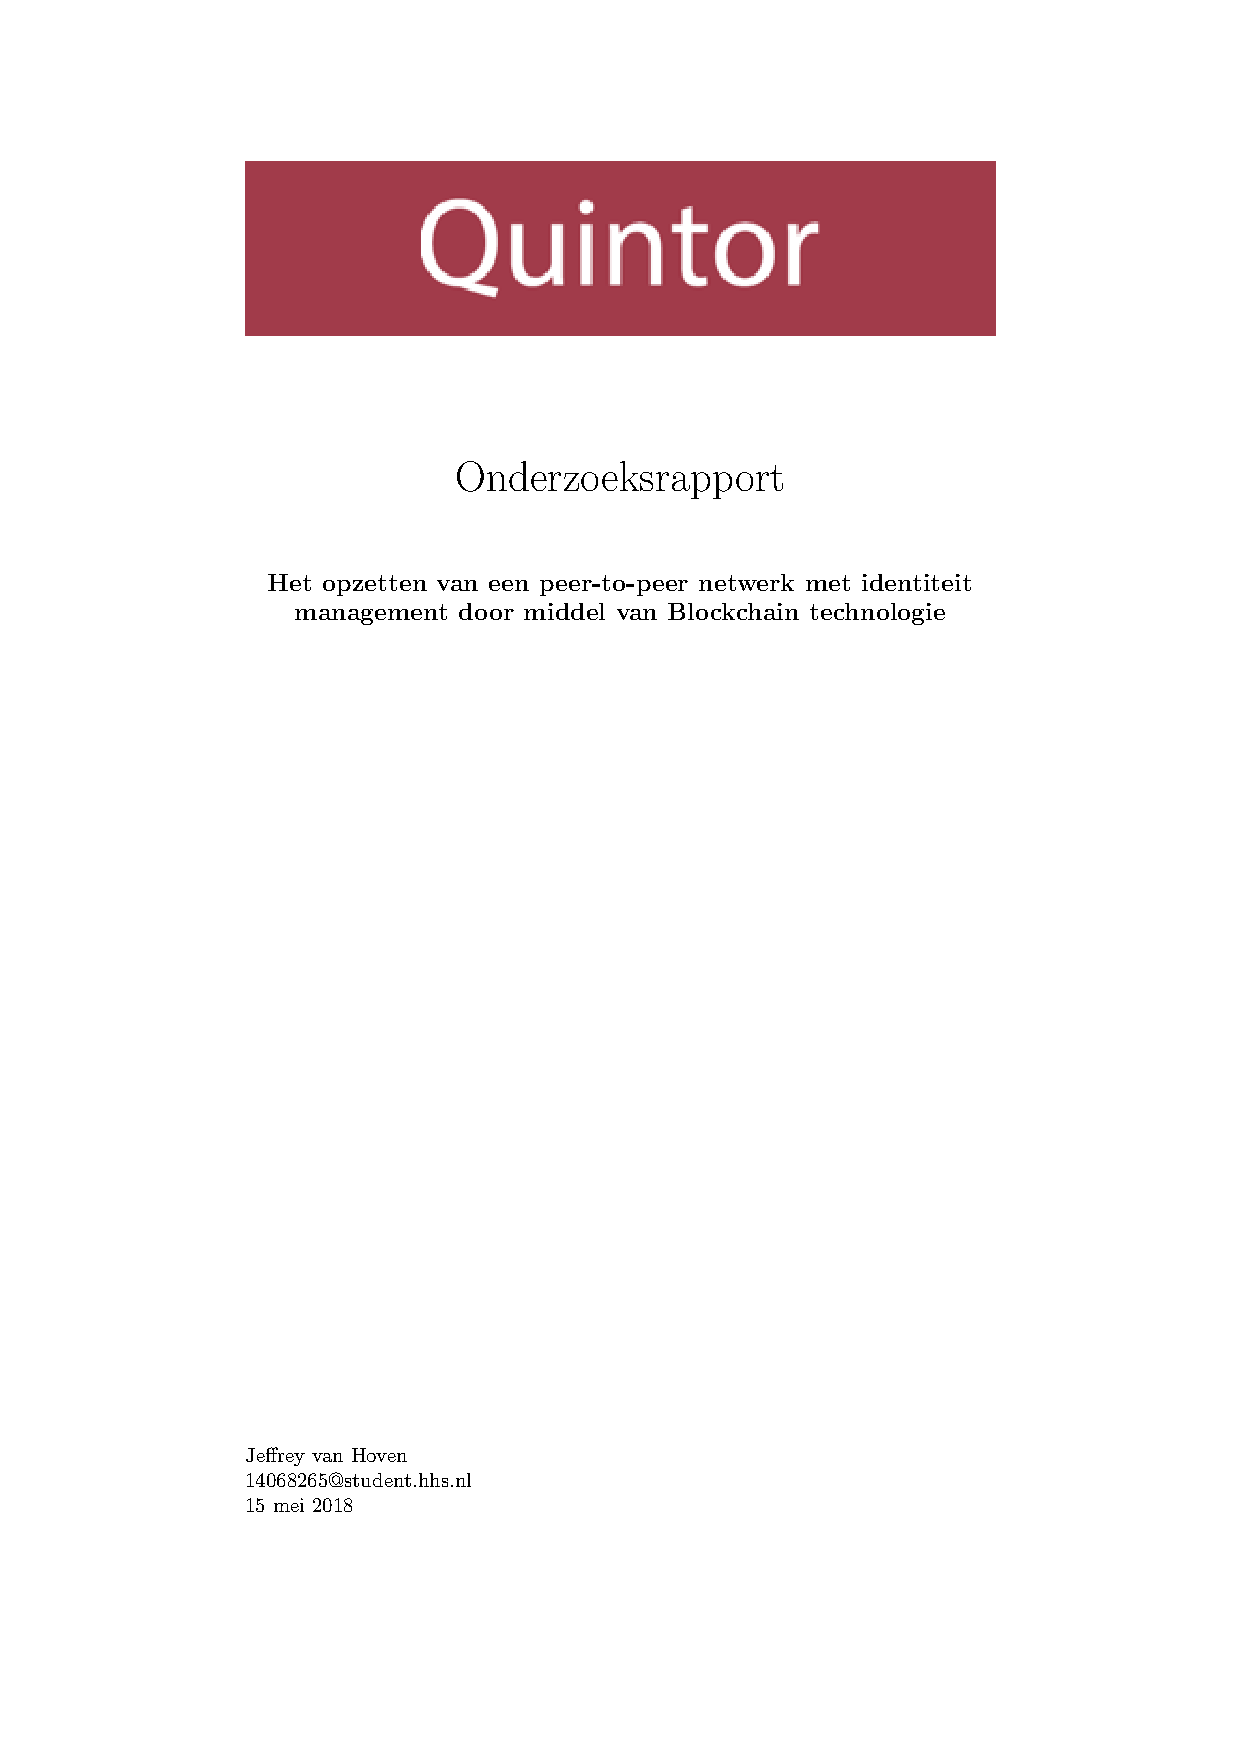
\includepdf[pages=-, frame=true, scale=0.7]{bijlages/Onderzoeksrapport/Onderzoeksrapport.pdf}

  \section{Adviesrapport}
  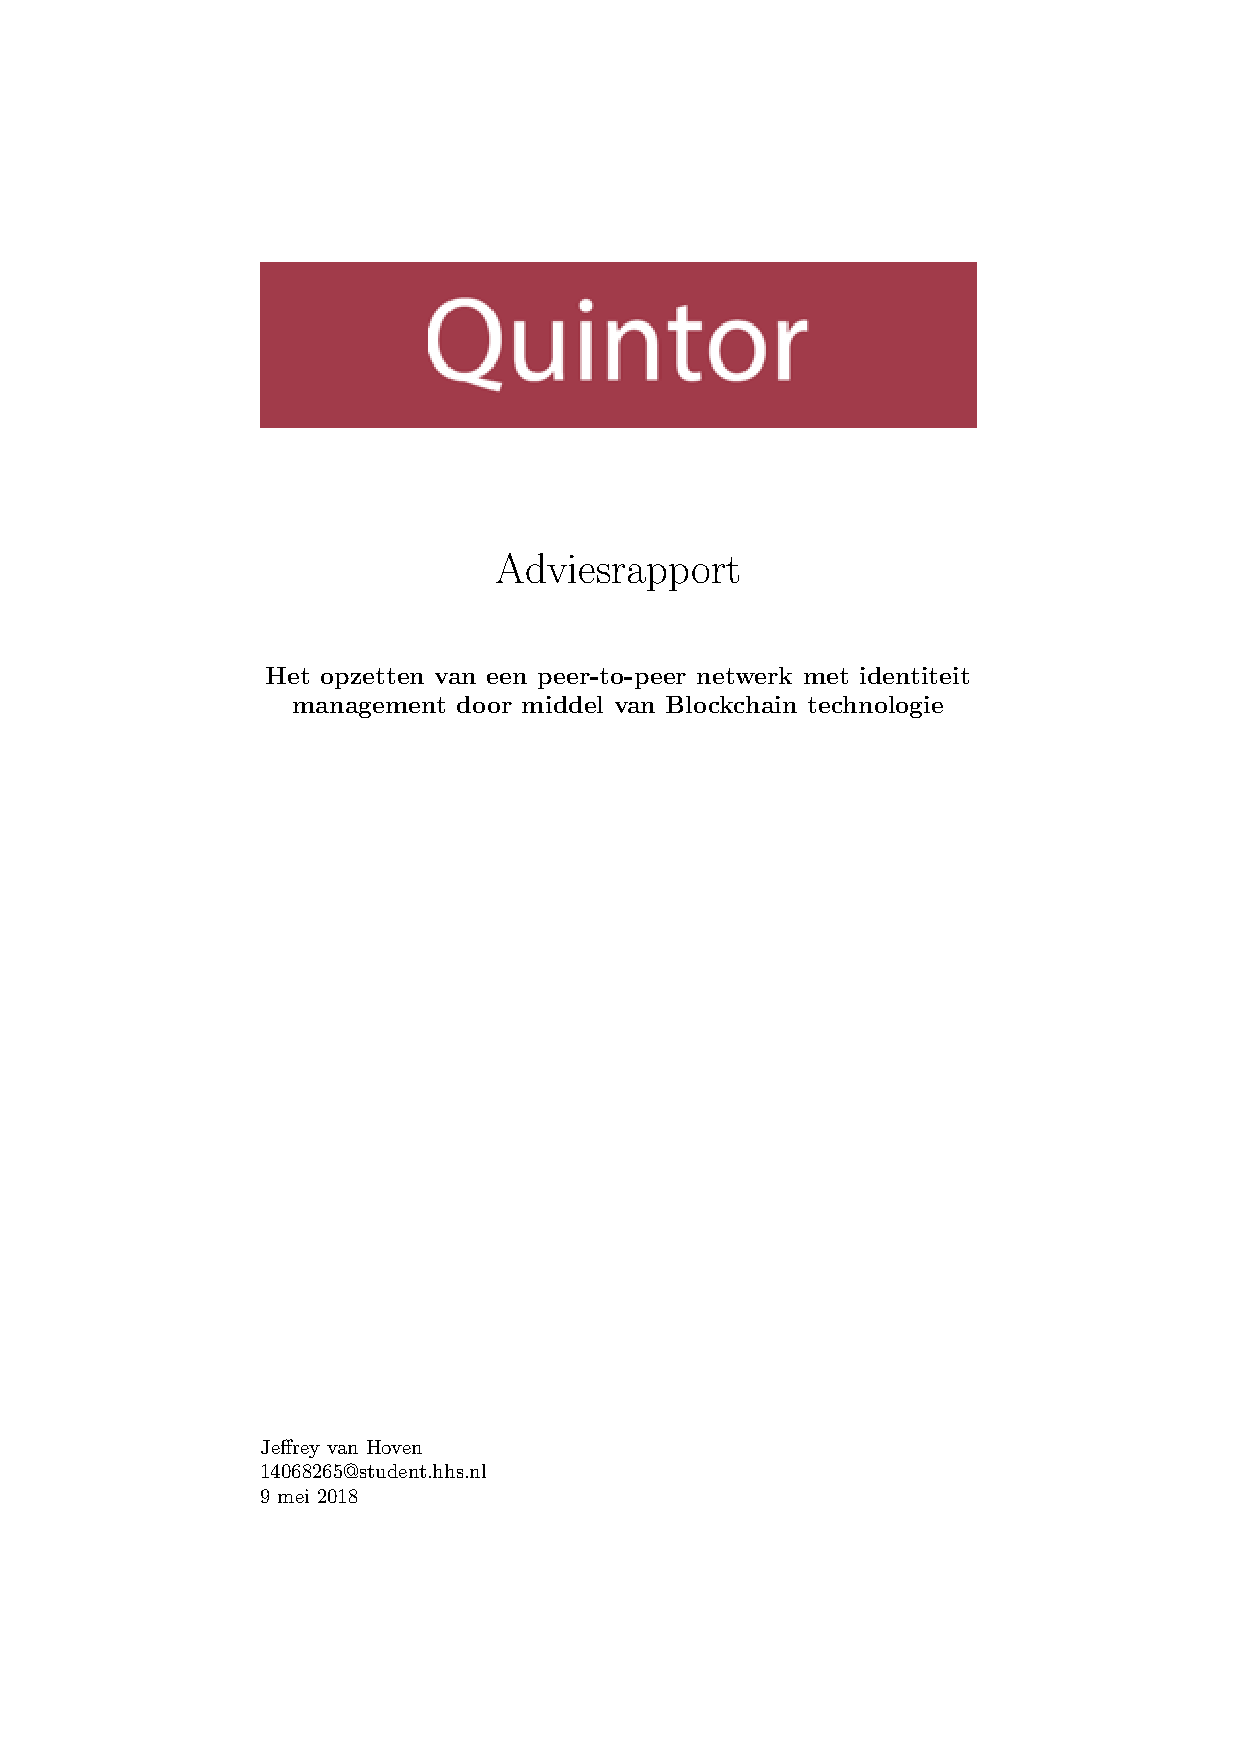
\includepdf[pages=-, frame=true, scale=0.7]{bijlages/Adviesrapport/Adviesrapport.pdf}

  \section{Voortgangsverslag}
  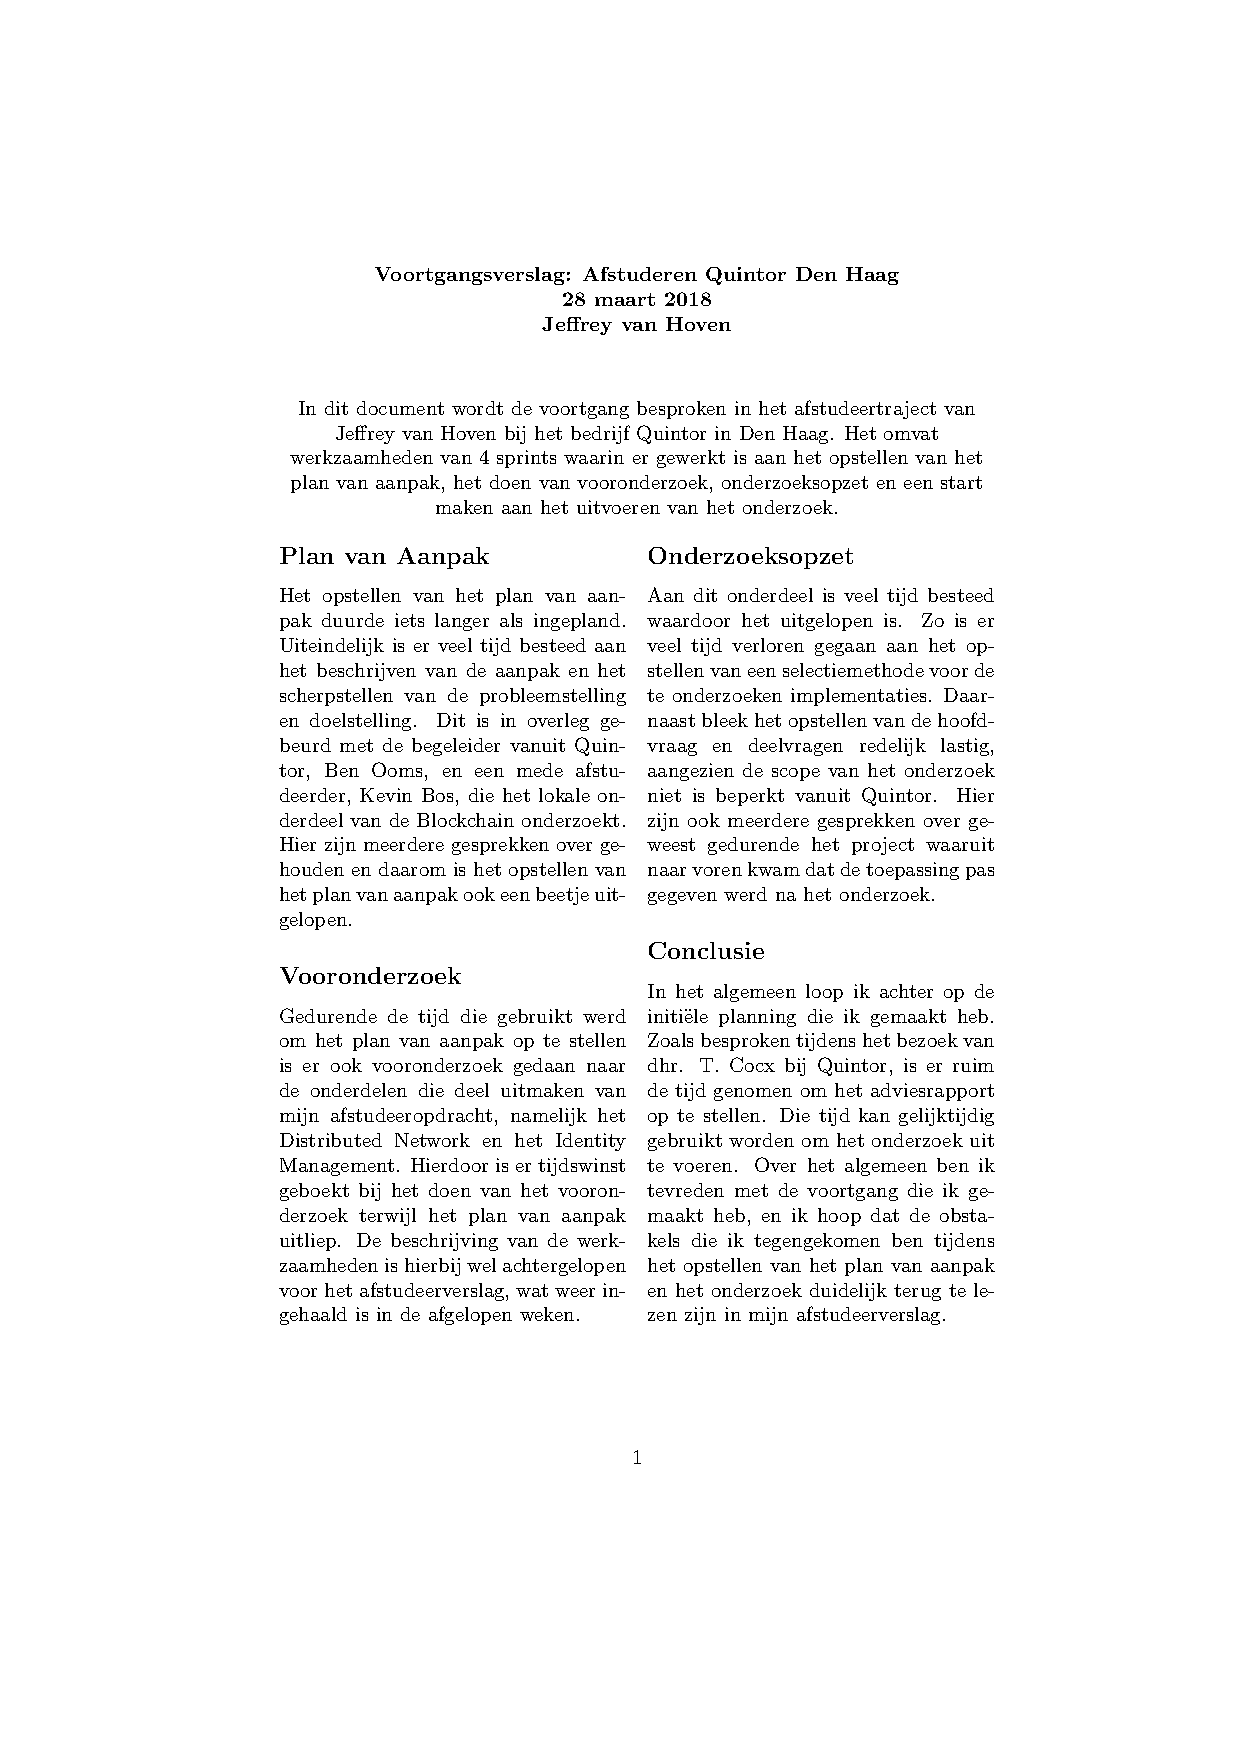
\includepdf[pages=-, frame=true, scale=0.7]{bijlages/Voortgangsverslag/Verslag.pdf}

  \section{Bezoekverslag}
  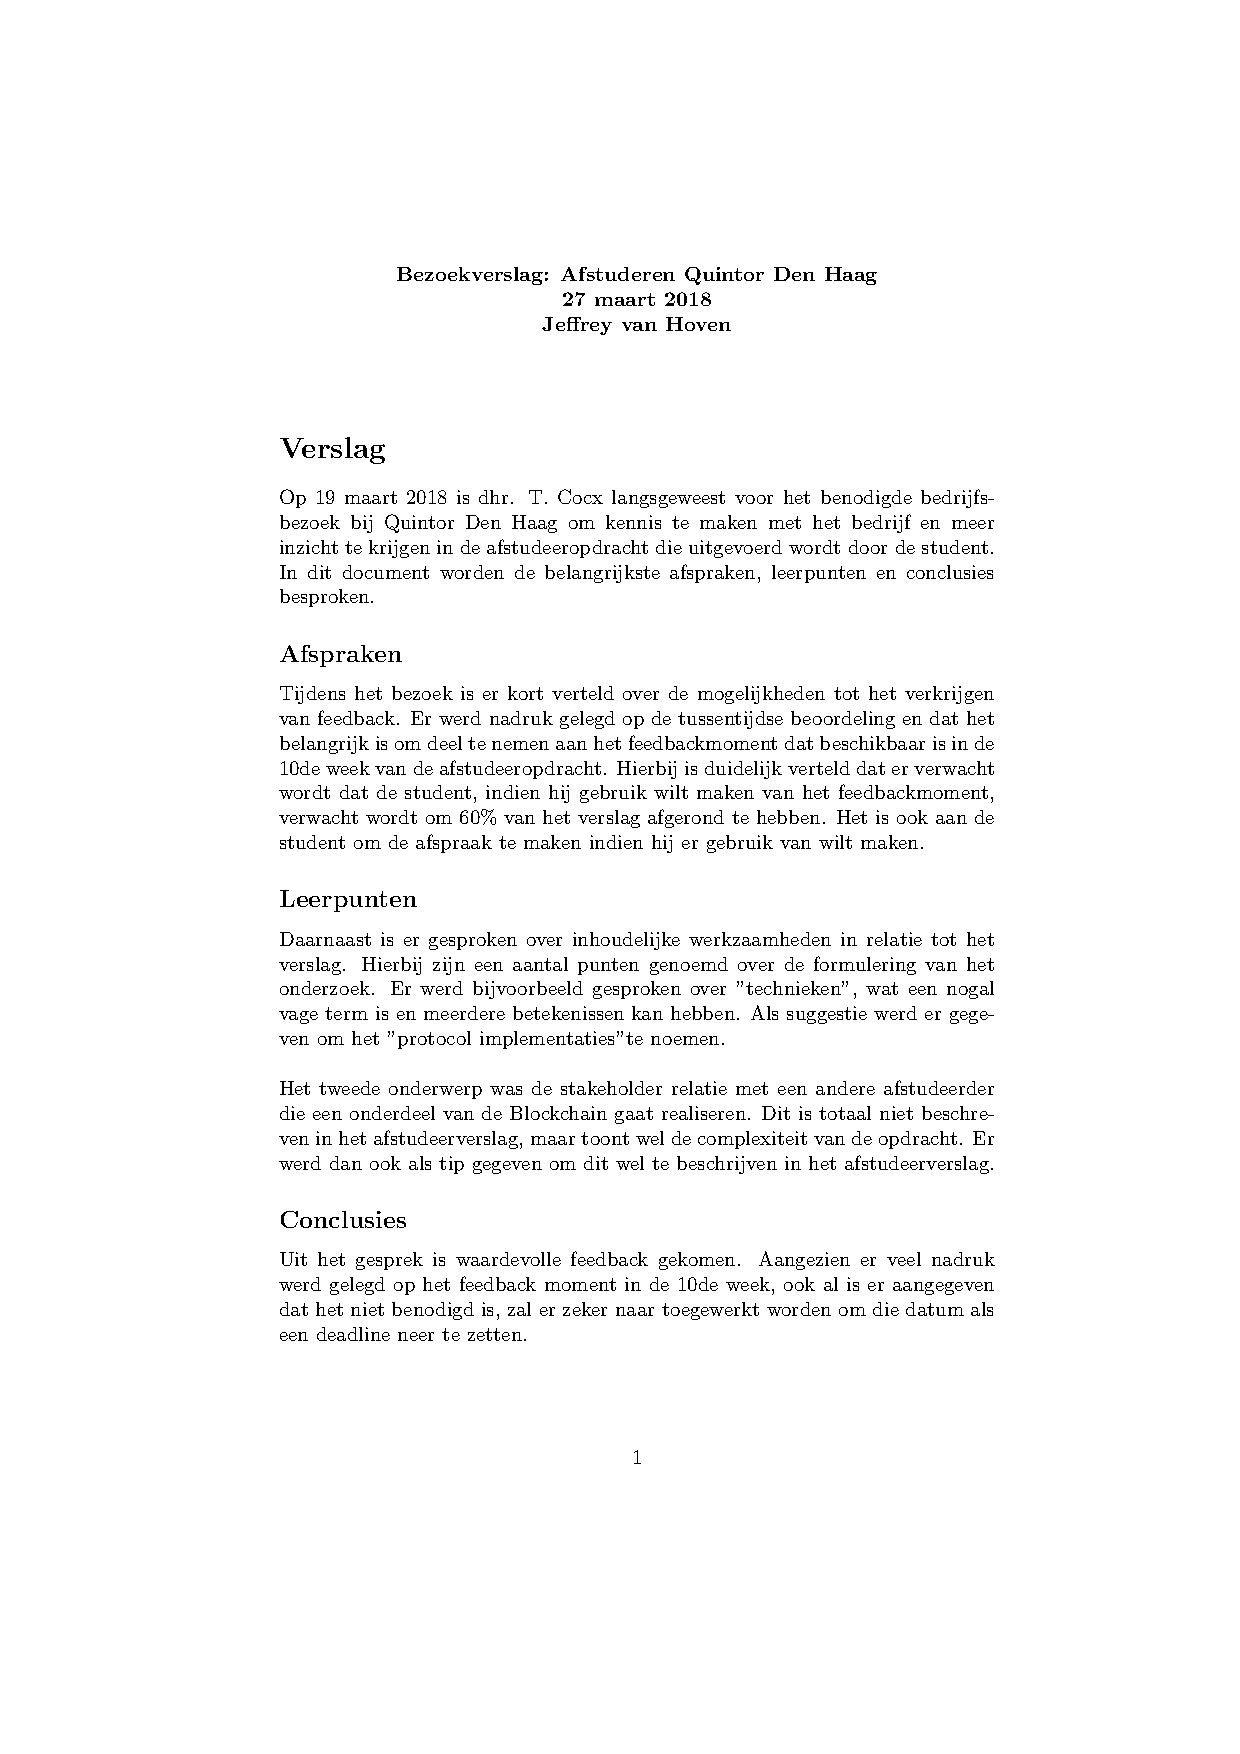
\includepdf[pages=-, frame=true, scale=0.7]{bijlages/Bezoek/Rapport.pdf}
  \addtocontents{toc}{\endgroup}
\end{appendices}
\end{document}
